\documentclass[12pt,letterpaper,english,bibliography=totocnumbered, abstract=on]{scrartcl}

\usepackage{indentfirst}
\usepackage[titletoc]{appendix}
\usepackage{fullpage}
%\usepackage{subfiles}
\usepackage[T1]{fontenc}
\usepackage[latin9]{inputenc}
\usepackage{color}
\usepackage{babel}
\usepackage{verbatim}
\usepackage[unicode=true,pdfusetitle,
bookmarks=true,bookmarksnumbered=false,bookmarksopen=false,
breaklinks=true,pdfborder={0 0 0},pdfborderstyle={},backref=false,colorlinks=true]
{hyperref}
\hypersetup{linkcolor=blue,citecolor=blue,urlcolor=blue}

\usepackage{booktabs}
\usepackage{multirow}
\usepackage{adjustbox}
\usepackage{threeparttable}
\usepackage[table]{xcolor}
\usepackage{csquotes}
\usepackage{soul} % for hiliting text: \hl

\usepackage[backend=biber, sorting=none]{biblatex}
\addbibresource{CRB.bib}
\addbibresource{extra.bib}

\usepackage{pdfpages}
\usepackage{float} % Allows use of H to place floats

\usepackage{pgfgantt}

\usepackage{framed}
\usepackage{todonotes}

\usepackage{gensymb}

\usepackage{subcaption}

\usepackage{siunitx}

% Prevent page breaks within paragraphs
% https://tex.stackexchange.com/questions/21983/how-to-avoid-page-breaks-inside-paragraphs
\widowpenalties 1 10000

\begin{document}

\titlehead{Final Report: DOI-OIA-D20AP00060}

\title{Establishment of Self-sustaining Biological Control of Coconut Rhinoceros Beetle Biotype G in Micronesia }

\author{Aubrey Moore PhD\\University of Guam College of Natural and Applied Sciences}

\date{February 29, 2024; Updated April 16, 2024}

\maketitle

\begin{description}
	\item[Reporting period] 2020-05-14 through 2023-12-31
\end{description}

Most recent online version: \\
\begin{footnotesize}	
	\url{https://github.com/aubreymoore/2020-FS-CRB-biocontrol-project/raw/master/fs-report-FINAL/doi-report-final-updated.pdf}
\end{footnotesize}

\clearpage

\tableofcontents

\clearpage


\newpage

\subsection*{Notes for the Reader}

\begin{itemize}

\item Each objective, as stated in the funded grant proposal \cite{mooreGrantProposalDOIOIA2020}, is presented in a frame at the start of each of the following sections. 

\item The University of Guam CRB biological control project is a long-term effort supported by multiple short-term grants.  

\end{itemize}

\clearpage

\section{Objective 1: Survey to Determine Background OrNV Incidence} 

\begin{framed}
CRB adults collected from breeding sites and pheromone traps throughout Guam will be tested for presence of OrNV using PCR.  Laboratory bioassays will be performed on OrNV isolated from these beetles to evaluate potential for biological control.
\end{framed} 

\subsection{Previously reported progress}

Our lab currently uses CRB-G adults collected from pheromone traps as test animals in bioassays to evaluate OrNV isolates as biocontrol agents under the assumption that the Guam beetle population contains only the CRB-G biotype and is free from OrNV infection. In 2019 we gained the capacity to perform PCR in our lab and began testing these assumptions. PCR results indicated that untreated, field-collected beetles, used as experimental controls in our bioassays, were all CRB-G, but 18\% of these tested positive for OrNV \cite{graselaTechnicalReportPolymerase2020, graselaTechnicalReportPolymerase2020a}.

Based on these results, the PI decided to suspend bioassays until we had conclusive evidence of OrNV infection in the Guam CRB-G population.  This decision was made for two reasons:

\begin{enumerate}
	\item If field-collected CRB insects where already infected with OrNV, these could not be used as test insects in laboratory bioassays designed to evaluate virulence of OrNV isolates.
	\item If an OrNV strain was already spreading within the Guam CRB population, it would be prudent to evaluate this strain as an effective biological control agent. 
\end{enumerate}

An experimental plan \cite{mooreExperimentalPlanDetermining2020} was developed and executed. One hundred beetles were collected from each of two pheromone trapping sites (Leo Palace Resort in Southern Guam and the UOG Ag. Expt. Stn. in northern Guam). Gut samples were obtained from these beetles and tested using PCR in our lab and also in Sean Marshall's lab at AgResearch New Zealand. 

In PCR results from both labs all beetles tested positive for CRB-G biotype and negative for OrNV infection \cite{graselaInvestigationDeterminePresence2020}. 

We concluded that previous OrNV positive tests were the result of lab contamination (not false positives). 

Current evidence suggests that all CRB on Guam belong to the CRB-G biotype and there is no OrNV infection within this population. In other words, the background OrNV incidence is zero.

\subsection{Recent progress}

Work on this objective has been completed. All evidence indicates that the OrNV incidence in the Guam CRB population is zero. We concluded that previous OrNV positive tests were the result of contamination in our lab. We have improved protocols to address this problem.

\clearpage
\section{Objective 2: Establish Sustainable CRB-G Biocontrol by Autodissemination of OrNV}

\begin{framed}
		
OrNV biocontrol candidates will be propagated \textit{in vivo} using established methods \cite{huger_oryctes_2005-1} and released into the Guam CRB-G population by autodissemination. Autodissemination involves infecting healthy CRB adults with OrNV. These infected beetles are then released at points dispersed throughout the island where they vector disease to conspecifics. A permit for field release of OrNV on Guam has already been obtained from USDA-APHIS. All released beetles will be marked by etching unique numbers on their elytra using a computer-controlled laser engraving system system already in use for this application at UOG.

Beetles for \textit{in vivo} propagation of OrNV and autodissemination will be field-collected from breeding sites and pheromone traps because this is far more efficient than rearing beetles in the lab at the current time. Impact of virus releases will be monitored using pheromone traps and a novel roadside video analysis system (see Objective \ref{monitoring}). A subset of beetles captured in traps will be used to estimate the virus infection rate. Concurrent with virus releases, we will continue to screen OrNV isolates to find candidate biocontrol agents.
\end{framed}


We have not made progress on this objective for two reasons:
\begin{enumerate}
	\item High mortality of untreated insects in experimental control groups and discovery of OrNV in some of these insects, presumably from laboratory contamination, have thrown results of previous bioassays into question.  We need to re-test several OrNV isolates we have previously evaluated in laboratory bioassays.
	\item We require permission from the US Environmental Protection Agency (USEPA) prior to release of OrNV as a biological control agent. Data demonstrating efficacy of OrNV as a biological control agent is required by USEPA.  
\end{enumerate}

We are currently reviewing our lab methods before resuming laboratory bioassays of OrNV isolates. We are considering changes to minimize OrNV contamination of samples in the bioassays and re-establishment of a CRB rearing program to provide high-quality test insects instead of relying on field-collected beetles.

\subsection{Recent progress}

We have revised our laboratory bioassay protocols. Previously, we used adults collected from pheromone traps as test insects. This source did not produce high quality, standardized adults needed for bioassays because these beetles were of unknown age and some were infected with pathogens or had other health problems. This caused high variability and high experimental control group mortality in our bioassay results. We now rear CRB from egg to adult in a dedicated CRB rearing lab using a natural diet we have developed. Adults produced by this lab are healthy, pathogen free and of a known age.

\paragraph{Development of a natural diet for CRB rearing.}

Previously, we individually reared CRB from egg to adult by placing them in Mason jars filled with a commercial steer manure/soil blend purchased from local hardware stores. However this is risky because manure may contain persistent pesticides fed to cattle or pesticides applied to the manure for fly control. 

We decided to eliminate this risk by making our own rearing diet from dead standing coconut stems which have begun to rot. We preferentially harvested stems naturally infested CRB grubs.

Processing is simple:
\begin{enumerate}
	\item Dead standing coconut stems are felled and bucked into 4 foot lengths
	\item Logs are run through a chipper and chips are loaded into burlap bags. Bags are placed in a chest freezer until needed.
	\item Chip size is reduced in an industrial Waring blender
	\item Material is loaded into Mason jars. This filled jars are sterilize using an autoclave
\end{enumerate}

\paragraph{Establishment of a CRB rearing lab.}

We converted a 40 foot shipping container into a CRB rearing lab. Temperature is maintained at 80\degree F by two independent air conditioners. Insects are reared individually from egg to adult by placing them in Mason jars filled with a natural rearing medium made from chipped standing dead coconut stems. There is shelf space for more than 2,000 jars (Fig. \ref{fig:rearing-lab}).

% TODO: \usepackage{graphicx} required
\begin{figure}[h]
	\centering
	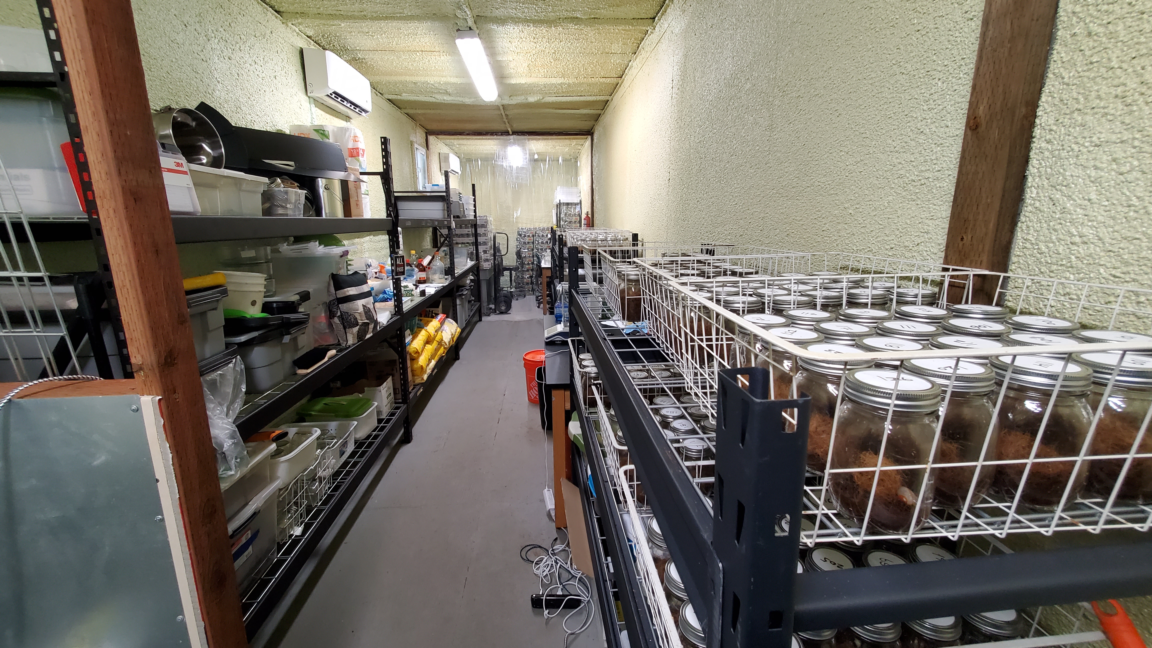
\includegraphics[width=\linewidth]{images/rearing-lab}
	\caption{Coconut rhinoceros beetle rearing lab at the University of Guam.}
	\label{fig:rearing-lab}
\end{figure}


\paragraph{Bioassays to determine sublethal effects of OrNV.}

Sublethal affects of OrNV infection may be much more important for CRB population suppression than direct mortality. A lab bioassay reported by Prasad et al. 2008 \cite{prasadManagementCoconutRhinoceros2008} showed that a high dosage of OrNV reduced the number of eggs laid per female from a mean of 58.5 to zero (100\% reduction in fecundity). Remarkably, when this dosage was reduced by a factor of 1000, the number of eggs laid per female was reduced from a mean of 58.5 to 16.5 (71.8\% reduction in fecundity).

We are preparing to repeat thus experiment using OrNV isolate V23B against CRB-G adults produced by our rearing lab. Isolate V23B is of particular interest because this isolate has been shown to infect CRB-G by our lab and also by independent research with CRB-G in the Solomon Islands \cite{barreraElectronMicroscopyStudy2021}. 

If the V23B isolate significantly reduces fecundity, we will use the results as evidence of efficacy as required by the US Environmental Protection Agency in support of a field application permit.

Our rearing facility is now starting to produce adults and bioassays will begin soon.

\clearpage

\subsection{Bioassays of Raw CRB Gut Samples from Palau}

\subsubsection{Objective}

The objective of this experiment is to see if CRB-G adults on Guam become infected with OrNV after being dosed with gut material dissected from CRB adults in Palau, were the natural OrNV infection rate is about 70\% (Kitalong, personal communication).

Each beetle in a treatment group will receive a single dose of a pooled sample of gut material applied to a banana slice. An experiment control group of beetles will be fed untreated banana slices.

The response variable will be longevity.

\subsubsection{Materials and Methods}

\paragraph{Gut Samples}
Gut samples dissected from CRB adults collected from Babeldaub, Palau were placed in Eppendorf tubes, frozen and brought to UOG by Dr. Chris Kitalong on November 11, 2022. These were stored in a household freezer at about -20 degrees C. Gut samples were crude with many containing male genitalia or eggs.

\paragraph{Test Insects}
CRB adults were collected from pheromone traps at Leo Palace Golf course, Guam December 2, 2022. These were placed individually into one pint Mason jars containing moist coir (CocoBrick). Each Mason jar was labeled with a unique integer serial number. Beetles were left unfed until the start of the bioassay.

\paragraph{Treatment}

Beetles were dosed by diet inclusion on December 6, 2022.  The gut sample within each Eppindorf tube was macerated using a toothpick. 
The toothpick was then used to transfer the sample into in a mortar containing small amount of water. A new toothpick was used to process each tube. After gut material from all Eppendorf tubes had been added to the mortar, this material was further macerated using a pestle. The macerate was transferred to a beaker and water was added to a total volume of 100 ml. Each beetle was dosed by dipping a banana slice into the beaker and placing this slice into the Mason jar containing the beetle. Half of the beetles were presented with untreated banana slices to provide an experimental control group. 

\paragraph{Observations}

Each beetle was observed every second day and fed a banana slice once a week. Each dead beetle was placed in a labeled sample container and stored in a domestic freezer at about -20 degrees C. Jars in which dead females had been kept were retained for 14 days at which time they were checked for larvae.

\paragraph{Post Mortem}

At the conclusion of the experiment, midguts were extracted, run through PCR, and tested for presence of OrNV using the methods of Tanaka \textit{et al.} 2021 \cite{tanakaConfirmationOryctesRhinoceros2021a}.Data for OrNV detection are recorded in \href{https://docs.google.com/spreadsheets/d/16k_lN9cihTnvhMoP54xnTwzWUBTzk1yDP79HW02dy5M/edit#gid=784130063}{this Google spreadsheet} in the \textbf{Aubrey's experiment} tab.

\paragraph{Analysis}

Data and Jupyter notebooks used for analysis are available in \href{https://github.com/aubreymoore/palau-guts-experiment}{this public GitHub repository}. 

\subsubsection{Results}

\paragraph{Mortality} Difference between mortality curves of treated and untreated beetles was insignificant (Fig. \ref{fig:palau-bioassay-1-survival-curves}).
\begin{figure}[h]
	\centering
	\includegraphics[width=0.7\linewidth]{"images/Palau bioassay 1 survival curves"}
	\caption{Survival curves.}
	\label{fig:palau-bioassay-1-survival-curves}
\end{figure}

\paragraph{Fecundity} The difference in fecundity between treated and untreated females was insignificant (Table \ref{fecundity contingency table}). In addition. the difference in mean number of larvae produced by treated and untreated females was insignificant (Table \ref{larvae per female}).
\begin{table}[H]
	\centering
	\caption{Contingency table for fecundity. Difference between groups is not significant (Fisher's exact test; p = 0.36)}
	\label{fecundity contingency table}
	\begin{tabular}{lcc}
		\hline
		& females not producing larvae & females producing larvae \\
		\hline
		untreated group & 31 & 17 (35\%) \\
		virus-treated group & 18 & 16 (47\%)\\
		\hline
	\end{tabular}
\end{table}
\begin{table}[H]
	\centering
	\caption{Number of larvae produced per female. Difference between group means is not significant (independent t-test; p = 0.56)}
	\label{larvae per female}
	\begin{tabular}{lcc}
		\hline
		& n & mean larvae per female \\
		\hline
		untreated group & 48 & 1.00 \\
		virus-treated group & 34 & 0.71 \\
		\hline
	\end{tabular}
\end{table}

\paragraph{OrNV detection} About a third of beetles in both treatment groups tested positive for OrNV (Table \ref{ornv detection}). This is an unexpected result.

\begin{table}[H]
	\centering
	\caption{OrNV detection.}
	\label{ornv detection}
	\begin{tabular}{lcc}
		\hline
		treatment & \multicolumn{2}{c}{OrNV detection} \\ \cline{2-3}
		          & Negative & Positive \\
		\hline
		control   & 26 & 15 (37\%)\\
		virus     & 29 & 15 (34\%)\\
		\hline
	\end{tabular}
\end{table}

\clearpage

\subsection{Bioassay of OrNV from Palau Prepared by the Tokyo University of Agriculture and Technology}

Note: This bioassay was designed and performed in collaboration with Mayuho Yamauchi, a visiting graduate student from the Tokyo University of Agriculture and Technology (TUAT).
A news story about this collaboration is available at:\\
\begin{tiny}
\url{https://www.uog.edu/news-announcements/2022-2023/2023-uog-tokyo-university-test-a-virus-on-guams-rhino-beetles.php}
\end{tiny}

\subsubsection{Objective}

This the major objective of this bioassay was to determine if there was a reduction in flight activity after dosing Guam CRB adults with an isolate of OrNV from Palau.

\subsubsection{Materials and Methods}

\paragraph{OrNV Samples}

The OrNV isolate used in this bioassay were collected from Palau and purified at TUAT.

\paragraph{Test Insects}

We used CRB adults collected from pheromone traps at the Leo Palace Resort on Guam.

\paragraph{Treatment}

Instead of treating individual we treated 4 cohorts of about 30 beetles each. Observations of individual insects were recorded using serial numbers etched on elytra using a laser marking machine. Each cohort was kept in an open 1 US gallon (3.8 liter) paint can half filled with moist cocopeat (Burpee Organic Seed Starting Mix). Cohorts were labeled A, B, C and D. Each paint can was kept in a large plastic garbage bin(Fig. \ref{fig:2023-uog-crb-moore-yamauchi-web}). Metal window screen covered the top of each bin. The lab air conditioner was set at 30 degrees C when no-one was working in it and all lights were turned off between 1800 h and 0600 h.

Beetles were fed by placing 30 grams of fresh banana paste on top of the cocopeat. Initial feeding dates were March 3 for cohort A, March 4 for cohort B, and March 5 for cohorts C and D. Beetles were fed weekly thereafter. 

Dosing was accomplished by incorporating 3.75 ml of the purified OrNV solution from TUAT into banana paste fed to cohorts C and D on the first feeding date (March 5).

\paragraph{Observations}

Each morning, beetles which had flown during the night were collected from the floor of each garbage bin and beetle serial numbers were recorded before they were returned to the paint cans. Mortality was checked daily. Dead beetles were stored in a freezer.

\paragraph{Post Mortem}

At the end of the experiment presence of OrNV was was determined using the methods of Tanaka \textit{et al.} 2021 \cite{tanakaConfirmationOryctesRhinoceros2021a}.

\paragraph{Analysis}

Data and Jupyter notebooks used for analysis are available in \href{https://github.com/aubreymoore/crb-flight-test}{this public GitHub repository}. 

% TODO: \usepackage{graphicx} required
\begin{figure}[H]
	\centering
	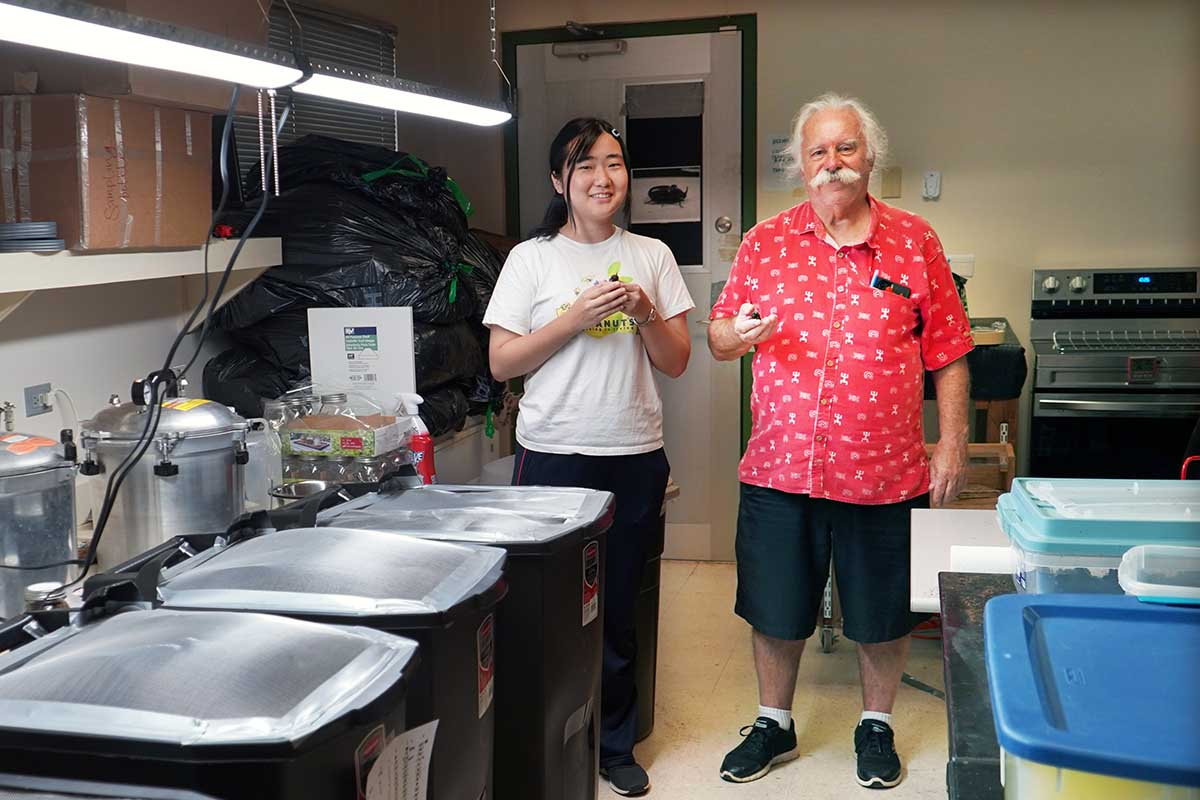
\includegraphics[width=\linewidth]{images/2023-uog-crb-moore-yamauchi-web}
	\caption{\textbf{Experimental setup.} Each of the garbage bins contained an open paint can, half filled with moist cocopeat in which CRB adults hid during the day. At 1800 h, overhead lights were turned off and beetles were able to fly out of the cans. Beetles which flew were collected at the bottom of the bins in morning.}
	\label{fig:2023-uog-crb-moore-yamauchi-web}
\end{figure}

\clearpage
\subsubsection{Results}

\paragraph{Mortality}

Difference between survival curves for virus-treated and untreated beetles was insignificant (Fig. \ref{fig:flight_test_survival_curves}).

% TODO: \usepackage{graphicx} required
\begin{figure}[H]
	\centering
	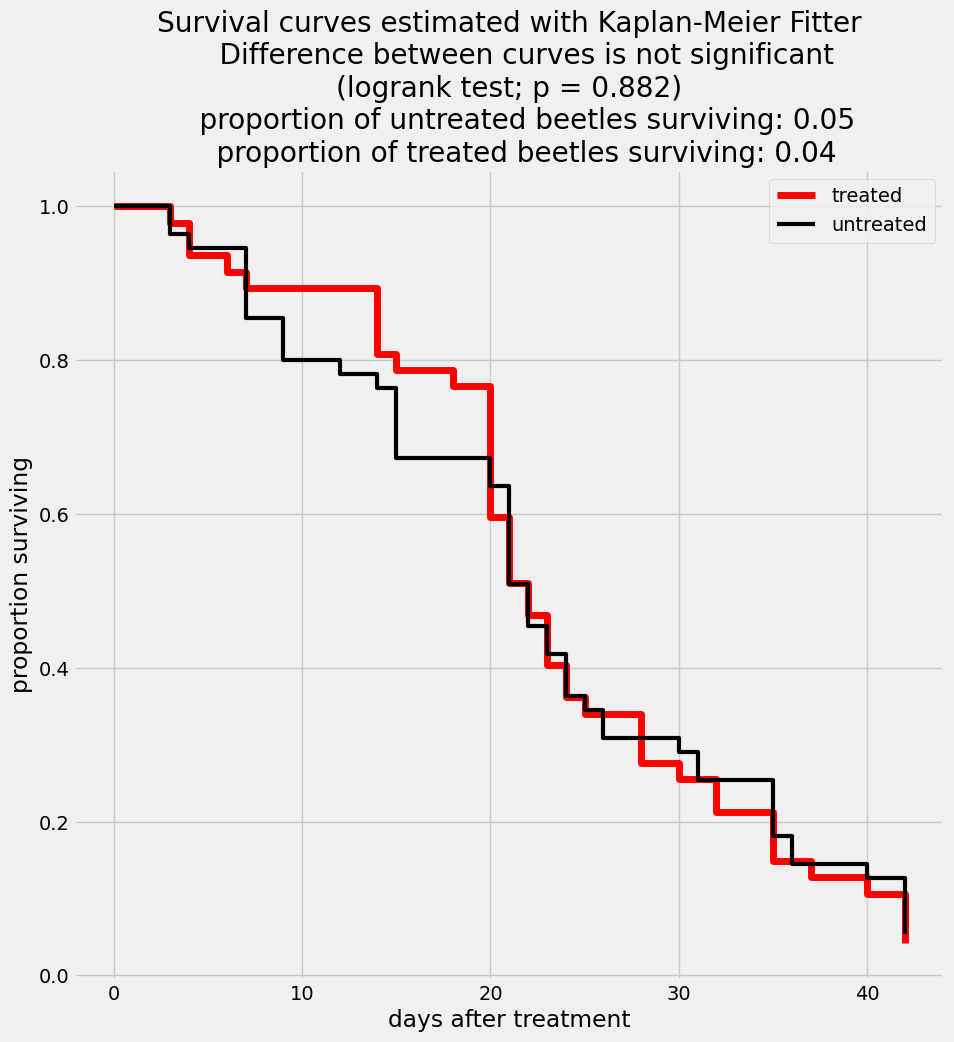
\includegraphics[width=0.7\linewidth]{images/flight_test/survival_curves}
	\caption{Survival curves}
	\label{fig:flight_test_survival_curves}
\end{figure}

\clearpage
\paragraph{Flight activity}.

% TODO: \usepackage{graphicx} required
\begin{figure}[H]
	\centering
	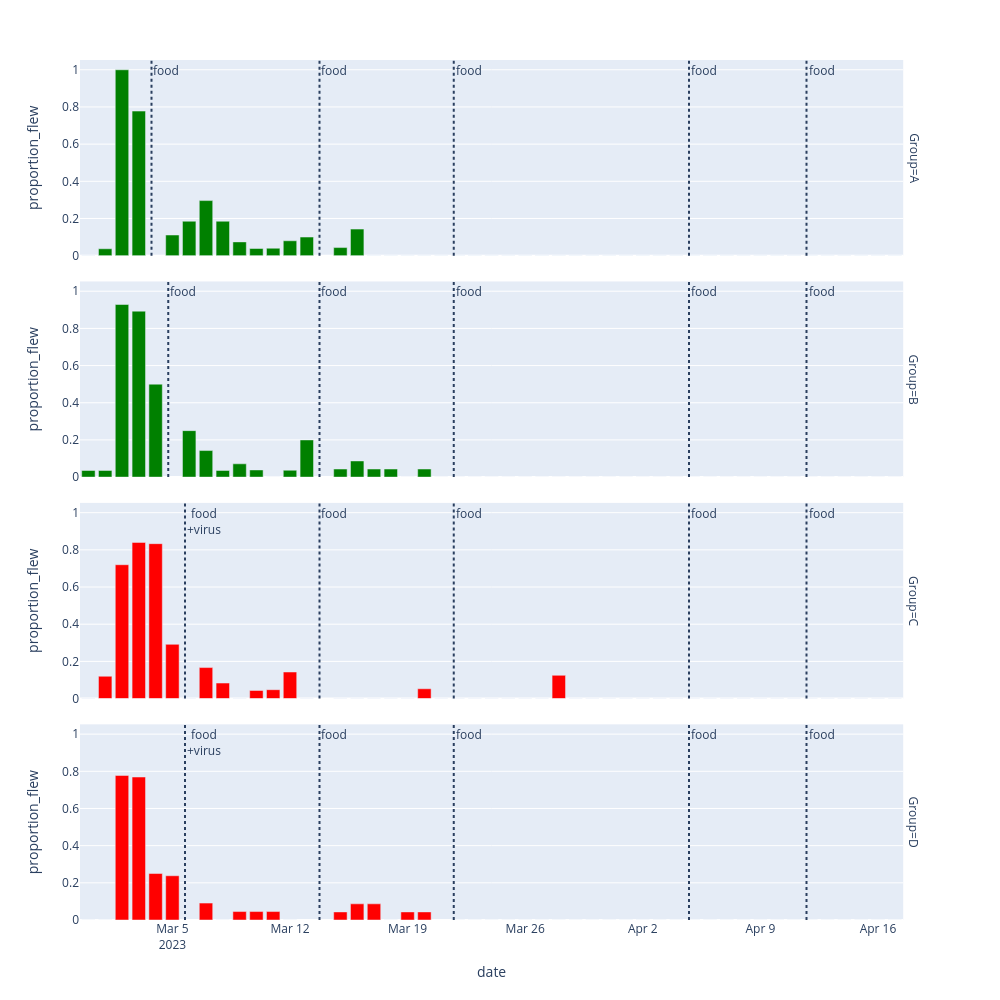
\includegraphics[width=0.7\linewidth]{images/flight_test/flight_activity}
	\caption{Flight activity.}
	\label{fig:flightactivity}
\end{figure}

\begin{table}[H]
	\centering
	\caption{\textbf{Flight activity.} Effect of treatment on flight activity was not significant. A Fisher exact test was applied to data for each date to test the hypothesis that flight activity was greater for beetles in the untreated control group. A combined p-value of 0.62 was calculated using Fisher's method.}
	\label{ornv detection}
	\begin{tabular}{l cc cc c}
		\toprule
		& \multicolumn{2}{c}{number of beetles which flew} & \multicolumn{2}{c}{number of beetles which did not fly} & \\
		\cmidrule(lr){2-3} \cmidrule(lr){4-5}		
		date       &  control         &  virus         &  control           &  virus           & p        \\
		\midrule
		2023-03-07 &               12 &              6 &                 45 &               46 & 0.1404 \\
		2023-03-08 &                6 &              2 &                 51 &               50 & 0.1672 \\
		2023-03-09 &                4 &              1 &                 51 &               50 & 0.2060 \\
		2023-03-10 &                2 &              2 &                 52 &               47 & 0.7271 \\
		2023-03-11 &                1 &              2 &                 53 &               47 & 0.8958 \\
		2023-03-12 &                3 &              3 &                 51 &               45 & 0.7154 \\
		2023-03-13 &                3 &              0 &                 46 &               47 & 0.1289 \\
		2023-03-15 &                2 &              0 &                 44 &               47 & 0.2419 \\
		2023-03-16 &                6 &              2 &                 40 &               45 & 0.1267 \\
		2023-03-17 &                1 &              2 &                 45 &               45 & 0.8750 \\
		2023-03-18 &                1 &              0 &                 44 &               47 & 0.4891 \\
		2023-03-19 &                0 &              1 &                 45 &               46 & 1.0000 \\
		2023-03-20 &                1 &              2 &                 43 &               41 & 0.8836 \\
		2023-03-28 &                0 &              1 &                 27 &               26 & 1.0000 \\
		\bottomrule
	\end{tabular}
\end{table}

\clearpage
\paragraph{Food consumption}

Differences in food consumption between untreated and virus-treated beetles were not significant.

\begin{figure}[H]
	\centering
	\begin{subfigure}{.49\textwidth}
		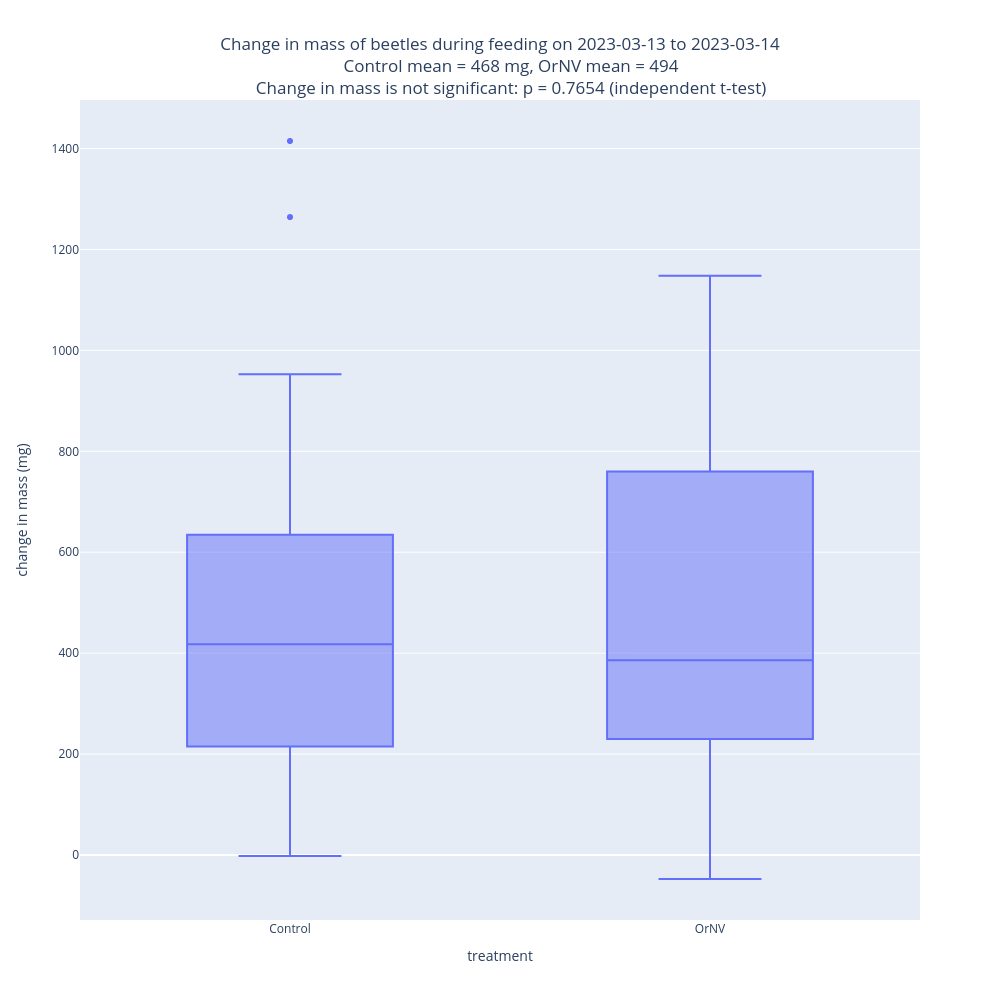
\includegraphics[width=\linewidth]{images/food_consumption_2023-03-13}
	\end{subfigure}
	%\hfill
	\begin{subfigure}{.49\textwidth}
		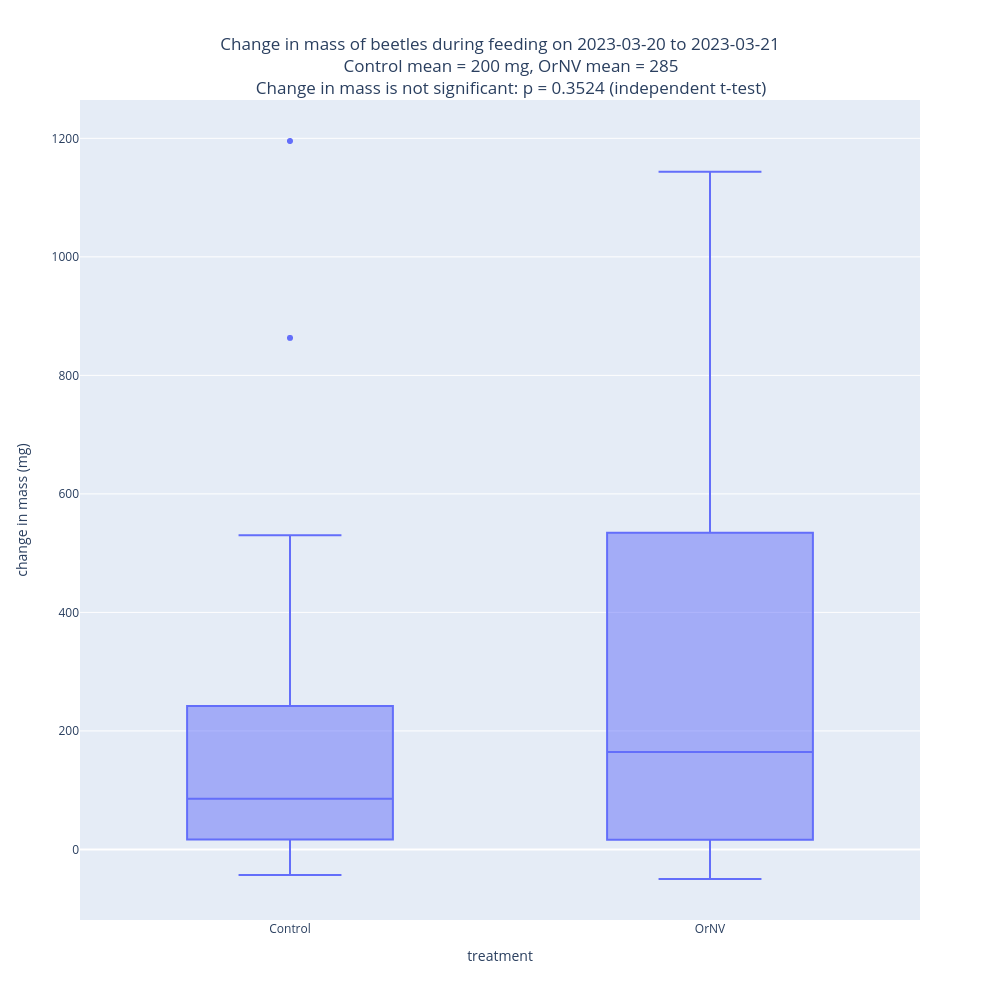
\includegraphics[width=\textwidth]{images/food_consumption_2023-03-20}
	\end{subfigure}
	%\hfill
	\begin{subfigure}{.49\textwidth}
		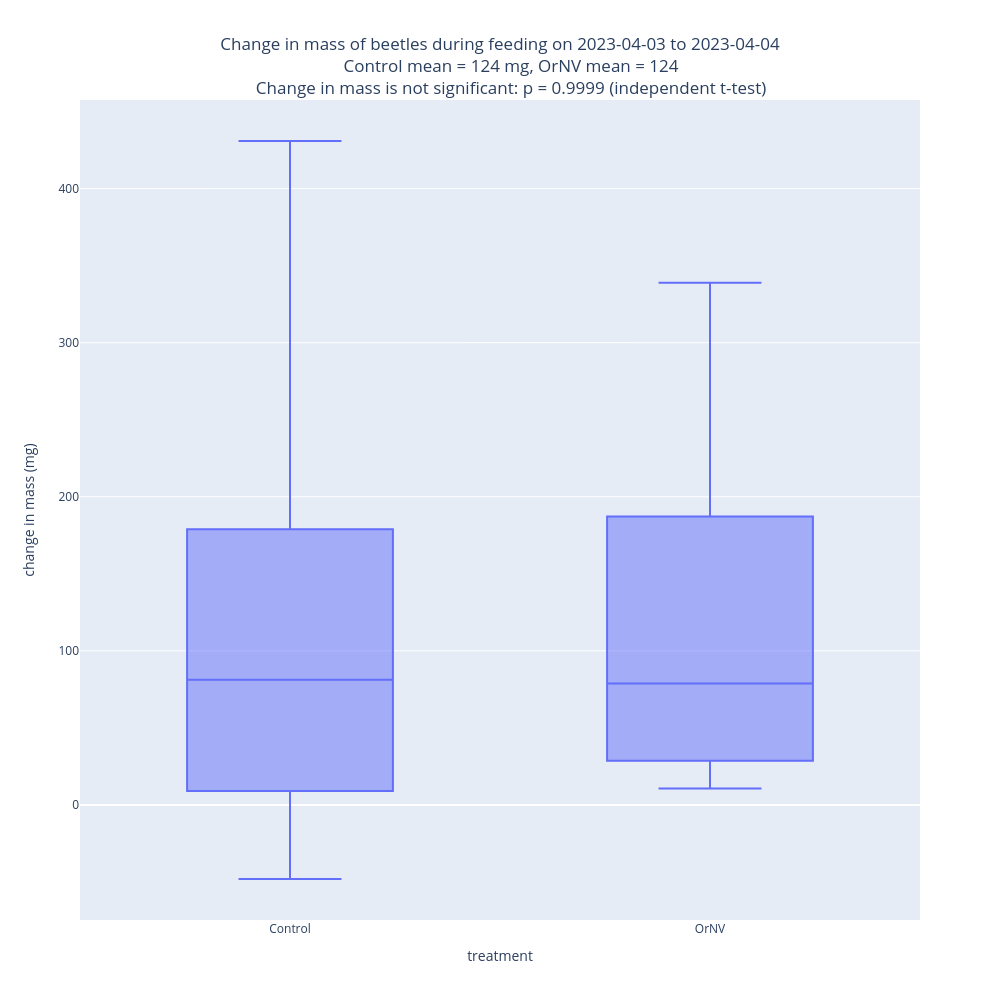
\includegraphics[width=\textwidth]{images/food_consumption_2023-04-03}
	\end{subfigure}
	%\hfill
	\begin{subfigure}{.49\textwidth}
		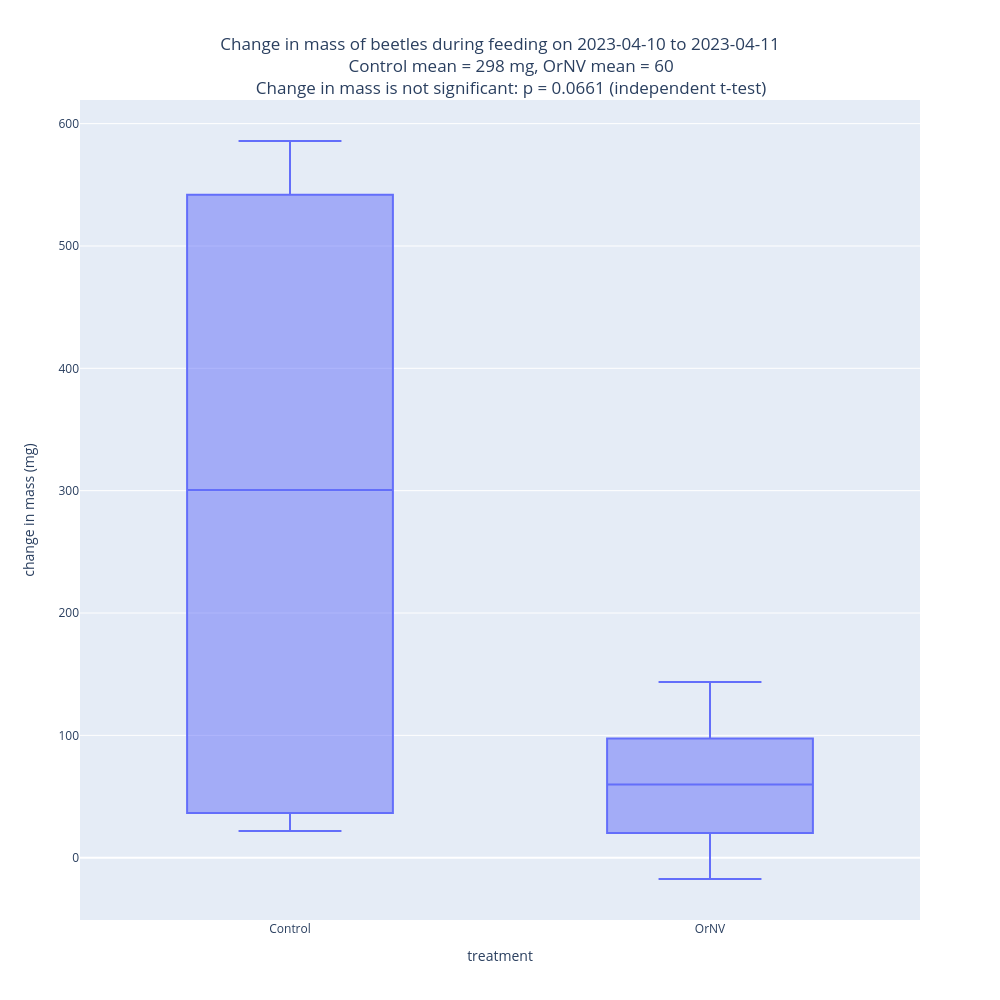
\includegraphics[width=\textwidth]{images/food_consumption_2023-04-10}
	\end{subfigure}
	\caption{Food consumption.}
	\label{fig:Palau2 food consumption}
\end{figure}

\clearpage
\paragraph{OrNV detection}.

\begin{table}[H]
	\centering
	\caption{OrNV detection.}
	\label{ornv detection}
	\begin{tabular}{lcc}
		\hline
		treatment  & \multicolumn{2}{c}{OrNV detection} \\ \cline{2-3}
		& Negative & Positive \\
		\hline
		control    & 15 & 0 ( 0\%)\\
		virus      & 14 & 3 (18\%)\\
		\hline
	\end{tabular}
\end{table}

\clearpage
\subsection{Bioassay of OrNV Isolates from AgResearch New Zealand}

\subsubsection{Objective}

The major objective of this bioassay was to assess four OrNV isolates as potential biological control agents for the Guam CRB population. 

\subsubsection{Materials and Methods}

\paragraph{OrNV Samples}

Purified OrNV samples labeled DUG42, PNG, V23B and X2B were provided by AgResearch New Zealand at a standardized titre of 1 x 10 6 infectious units per milliliter (IU/mL), with virus supplied in 1 mL aliquots. The minimum dose recommended to establish infection in a susceptible beetle is 5000 IU and a maximum challenge dose should be from 40,000 to 50,000 IU. \cite{AgResearch2023-OrNV-prep2023}.

\paragraph{Test Insects}

CRB adults were collected from pheromone traps at the Leo Palace Resort. Each beetle was kept in a Mason jar half filled with moist cocopeat (Burpee Organic Seed Starting Mix). Beetles were kept for 2 weeks prior to being used in the bioassay.

\paragraph{Treatment}

The standard method for dosing CRB adults with OrNV is to apply droplets of a sugar solution containing virus particles to the mouthparts using a pipette \cite{AgResearch2023-OrNV-prep2023,AgResearch2023-OrNV-minitest}. This droplet method was used to dose Guam beetles used in our first bioassay on 2023-07-31. However, very few beetles imbibed the target dose. As an alternative, we developed a tube method \cite{tube-dosing-method} where beetles were fed a 10\% sugar solution containing OrNV particles by placing them in Falcon tubes with so that their mouthparts were submerged in the solution (Fig. \ref*{fig:tubemethod}).

% TODO: \usepackage{graphicx} required
\begin{figure}[H]
	\centering
	\caption{\textbf{Tube method.} Beetles were dosed by immersing mouth parts in 2 ml of 10\% sucrose containing 1 million IU of OrNV.}
	\label{fig:tubemethod}
	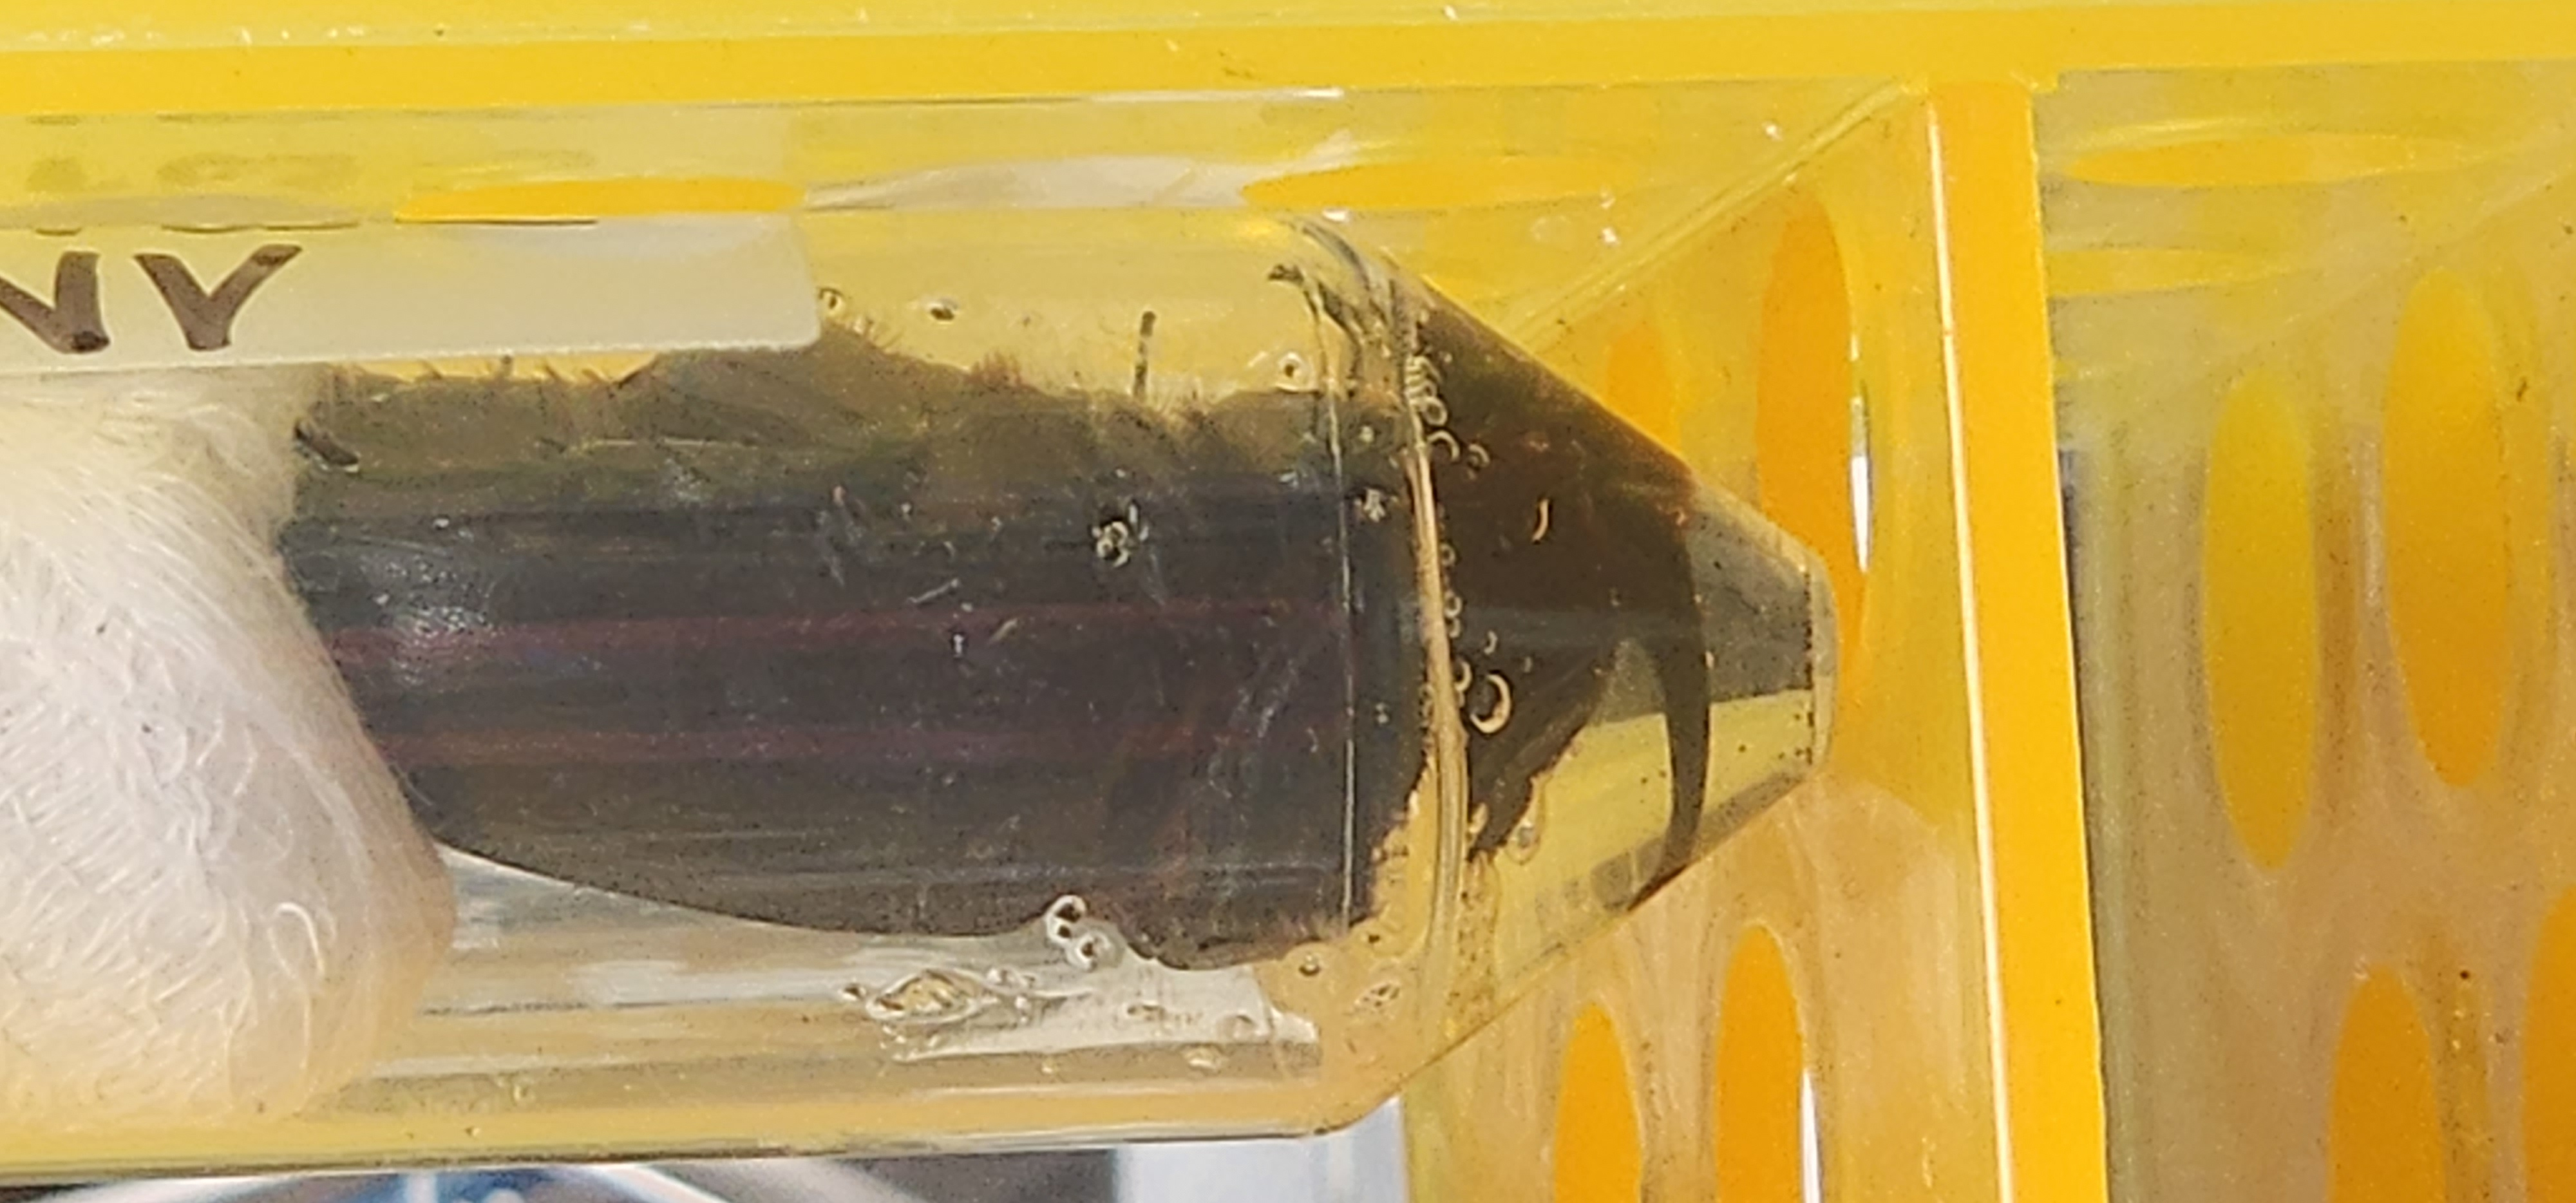
\includegraphics[angle=-90,origin=c,width=0.15\linewidth]{images/tube_method}
\end{figure} 

To prepare the dosing solution, we mixed 1 ml of virus solution with 1m of 20\% sucrose, resulting in a 10\% sucrose solution containing virus at a titre of 500 IU per microlitre (approximately equal to 500 IU per milligram). Thus, to acquire a target maximum challenge dose of 40,000 IU, a beetle would have to drink 80 milligrams of the solution. Each beetle was placed in a Falcon tube for 20 minutes. Dose was estimated by weighing the beetle before and after it was placed in the tube. During the bioassay, lab temperature was maintained at 85 \degree F (29.4 \degree C) when no-one was working in it (Fig. \ref{fig:lab}). 

% TODO: \usepackage{graphicx} required
\begin{figure}[H]
	\centering
	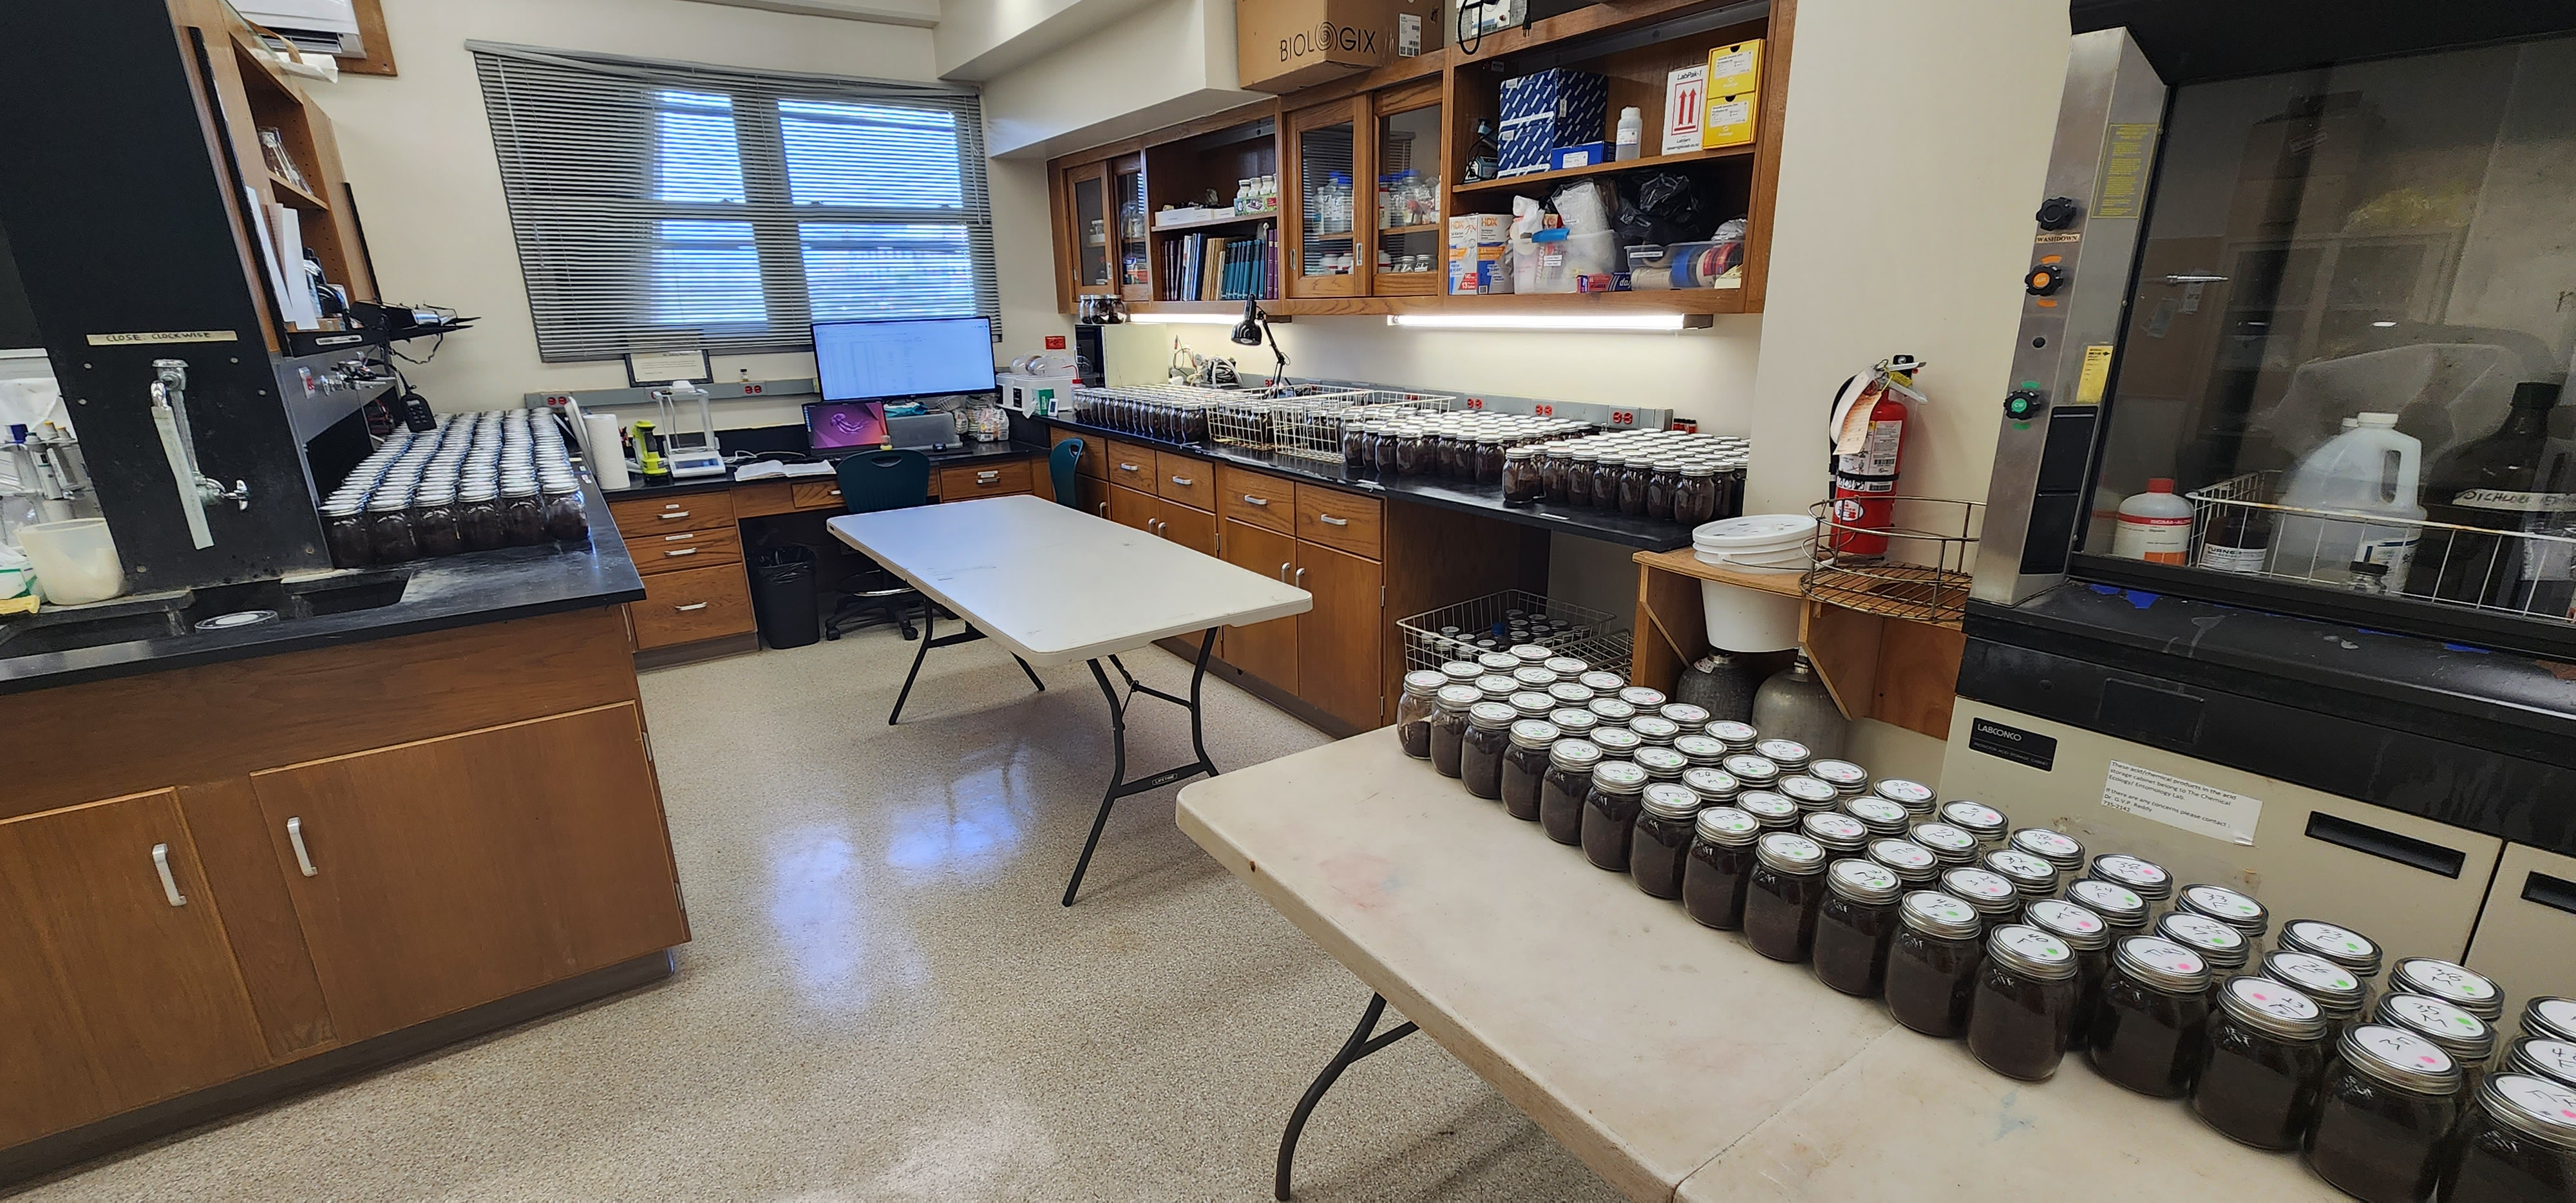
\includegraphics[width=0.7\linewidth]{images/lab}
	\caption{Each Mason jar contains a CRB adult in a OrNV bioassay.}
	\label{fig:lab}
\end{figure}

\paragraph{Observations}

Beetles were checked for mortality every day or second day. A postmortem was performed on each dead beetle on the day it was found.

\paragraph{Post Mortem}

Post mortems were performed using the standard method \cite{AgResearch2023-OrNV-minitest}. Beetles were considered to be dead when there was no leg movement. However, after elytra were removed, microscopic examination revealed that the dorsal heart was still beating in many specimens. During the post mortem examination each beetle was examined externally and internally under a stereozoom microscope to determine presence of mites and nematodes. Presence of a heartbeat was also recorded. An image of the mid gut of each beetle prior to excision was recorded with a cell phone camera. 
Excised midgut samples were shipped to AgResearch New Zealand for molecular analysis and histology.

\paragraph{Analysis}

Data and Jupyter notebooks used for analysis are available in \href{https://github.com/aubreymoore/ornv-bioassay-db}{this public GitHub repository}. 

\clearpage
\subsubsection{Results}

\paragraph{Mortality}.

% DUG42 survival curves.

\begin{figure}[h]
	\centering
	\begin{subfigure}{.3\textwidth}
		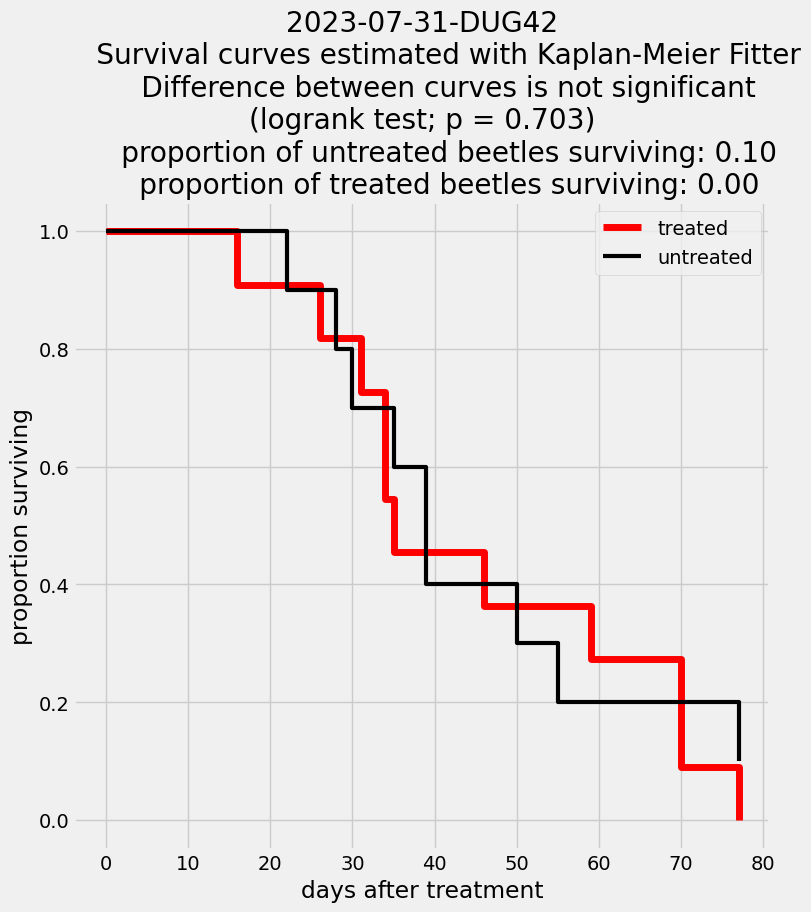
\includegraphics[width=\linewidth]{images/survival_curves/2023-07-31-DUG42}
		\caption{Replicate 1.}
	\end{subfigure}
	%\hfill
	\begin{subfigure}{.3\textwidth}
		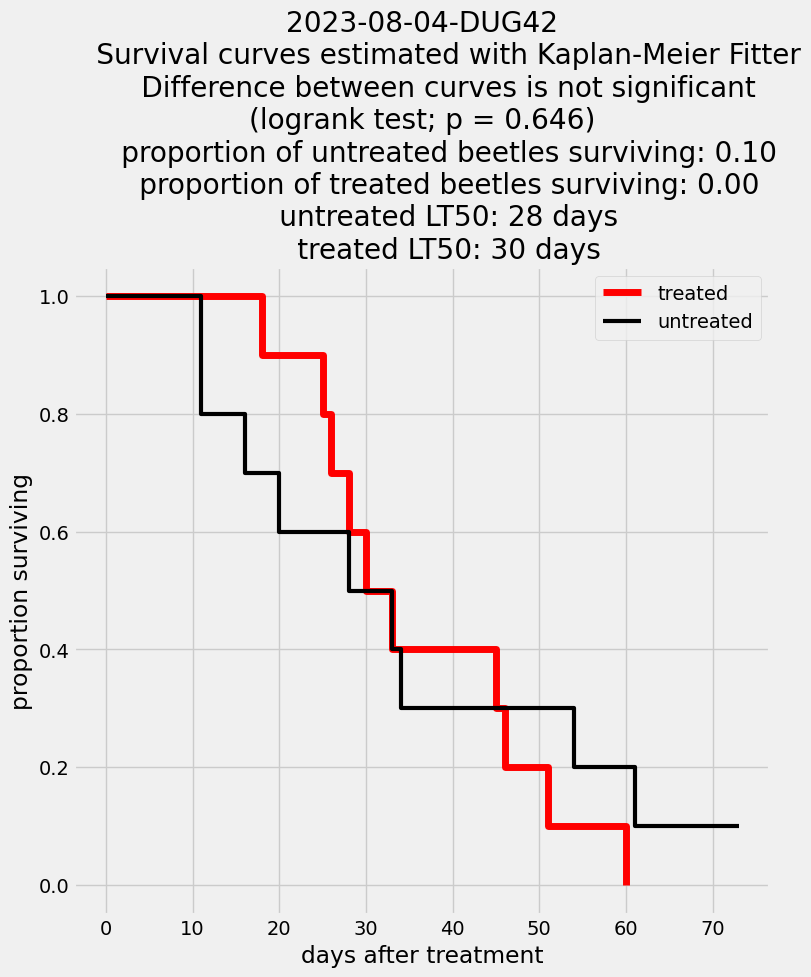
\includegraphics[width=\textwidth]{images/survival_curves/2023-08-04-DUG42}
		\caption{Replicate 2.}
	\end{subfigure}
	%\hfill
	\begin{subfigure}{.3\textwidth}
		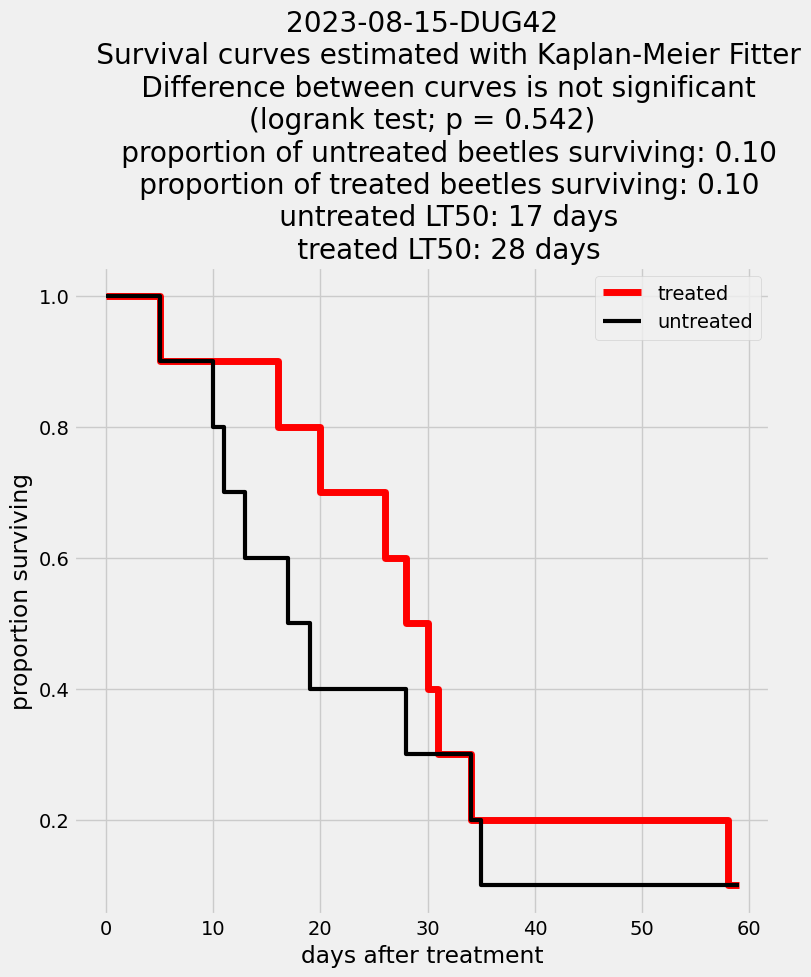
\includegraphics[width=\textwidth]{images/survival_curves/2023-08-15-DUG42}
		\caption{Replcate 3.}
	\end{subfigure}
	%\hfill
	\begin{subfigure}{.3\textwidth}
		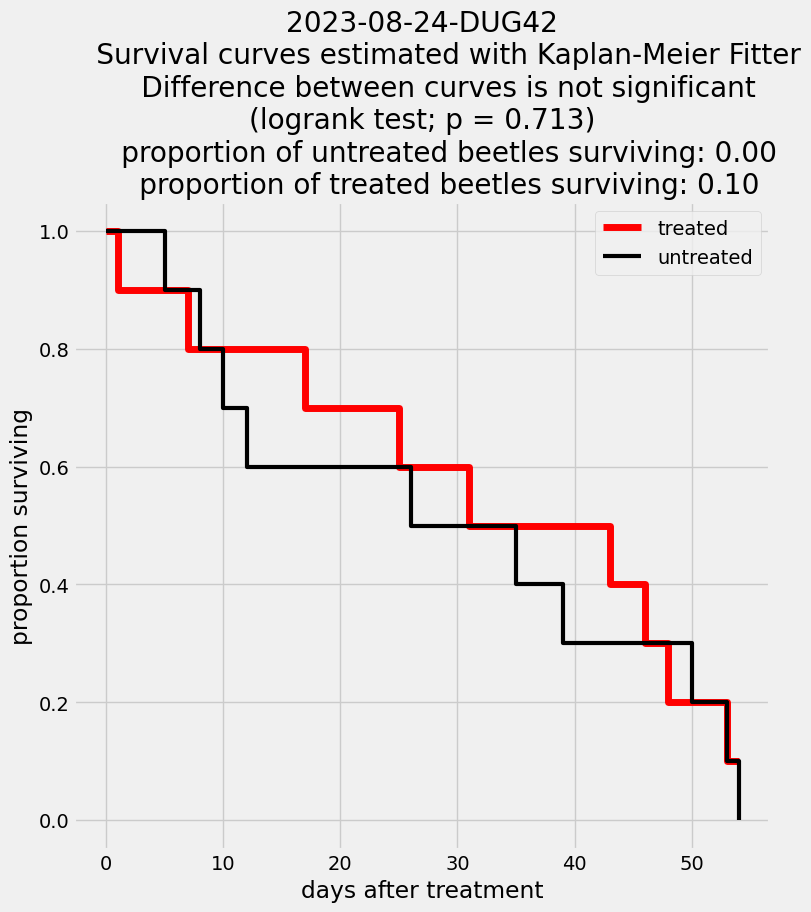
\includegraphics[width=\textwidth]{images/survival_curves/2023-08-24-DUG42}
		\caption{Replicate 4.}
	\end{subfigure}
	%\hfill
	\begin{subfigure}{.3\textwidth}
		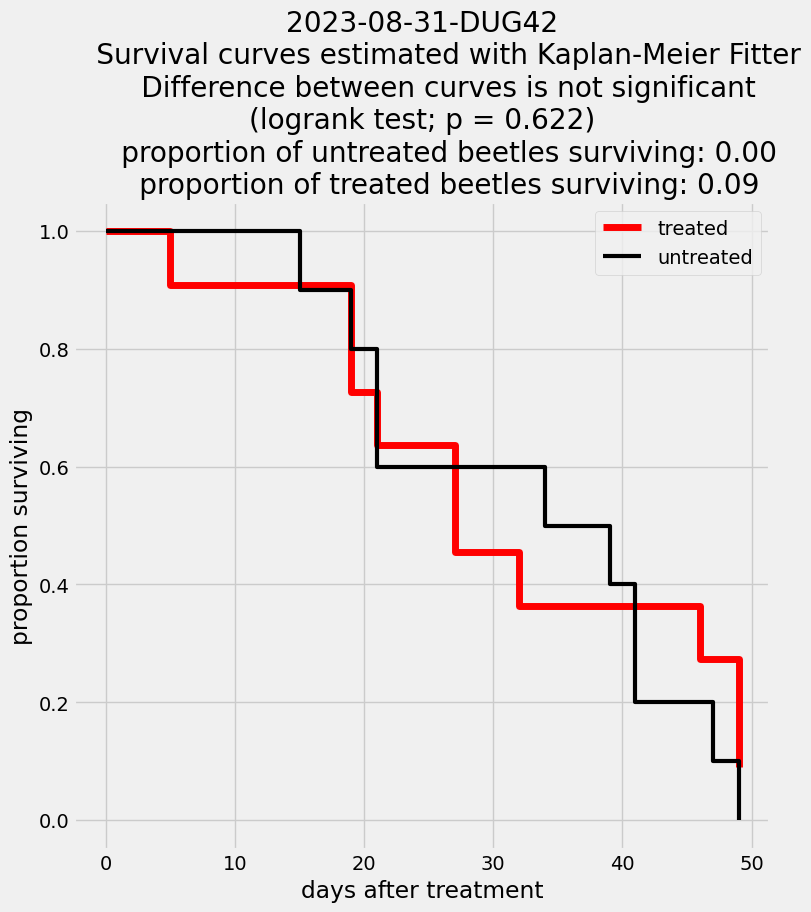
\includegraphics[width=\textwidth]{images/survival_curves/2023-08-31-DUG42}
		\caption{Replicate 5.}
	\end{subfigure}
	\caption{Survival curves for bioassays of OrNV isolate DUG42.}
	\label{fig:DUG42 survival curves}
\end{figure}

% PNG survival curves

\begin{figure}[h]
	\centering
	\begin{subfigure}{.3\textwidth}
		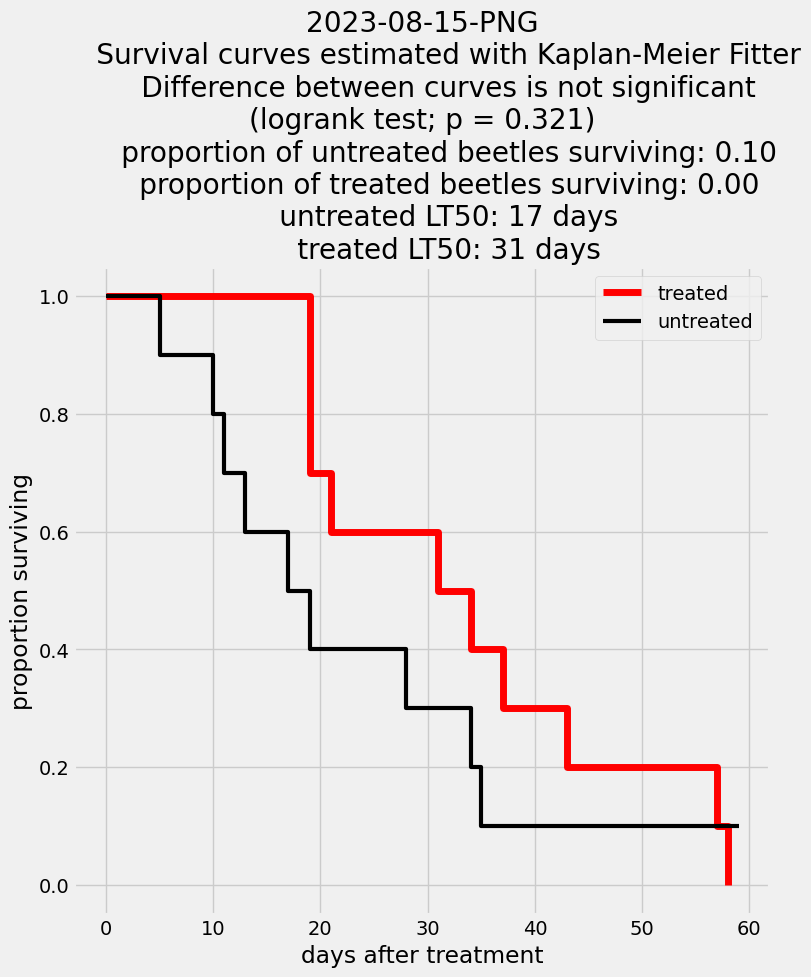
\includegraphics[width=\linewidth]{images/survival_curves/2023-08-15-PNG}
		\caption{Replicate 1.}
	\end{subfigure}
	\begin{subfigure}{.3\textwidth}
		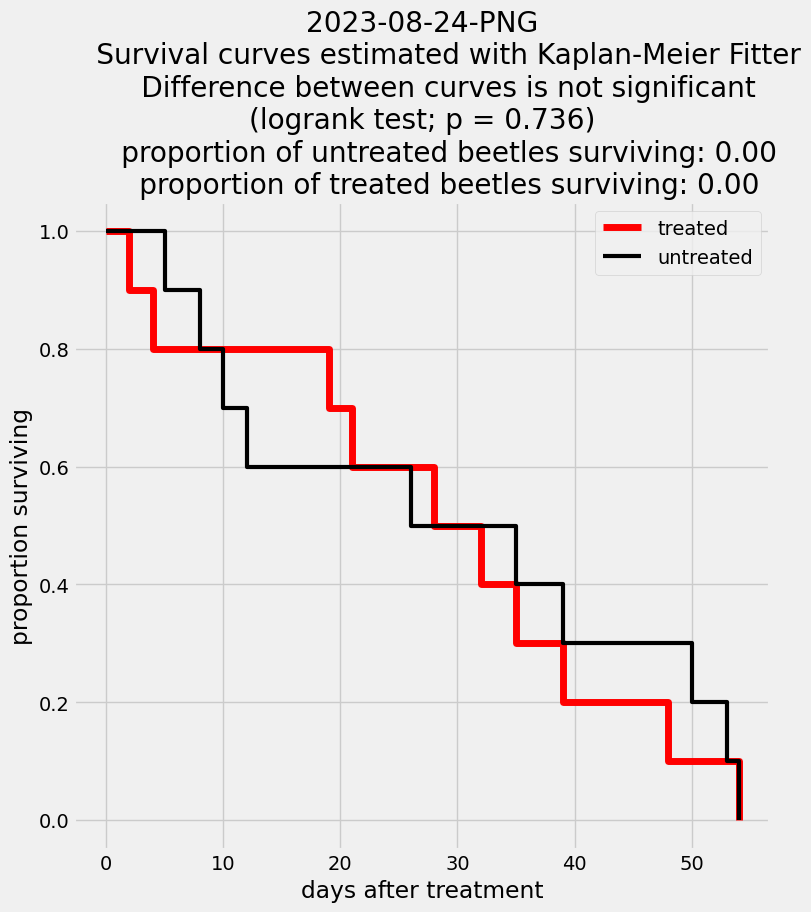
\includegraphics[width=\textwidth]{images/survival_curves/2023-08-24-PNG}
		\caption{Replicate 2.}
	\end{subfigure}
	\begin{subfigure}{.3\textwidth}
		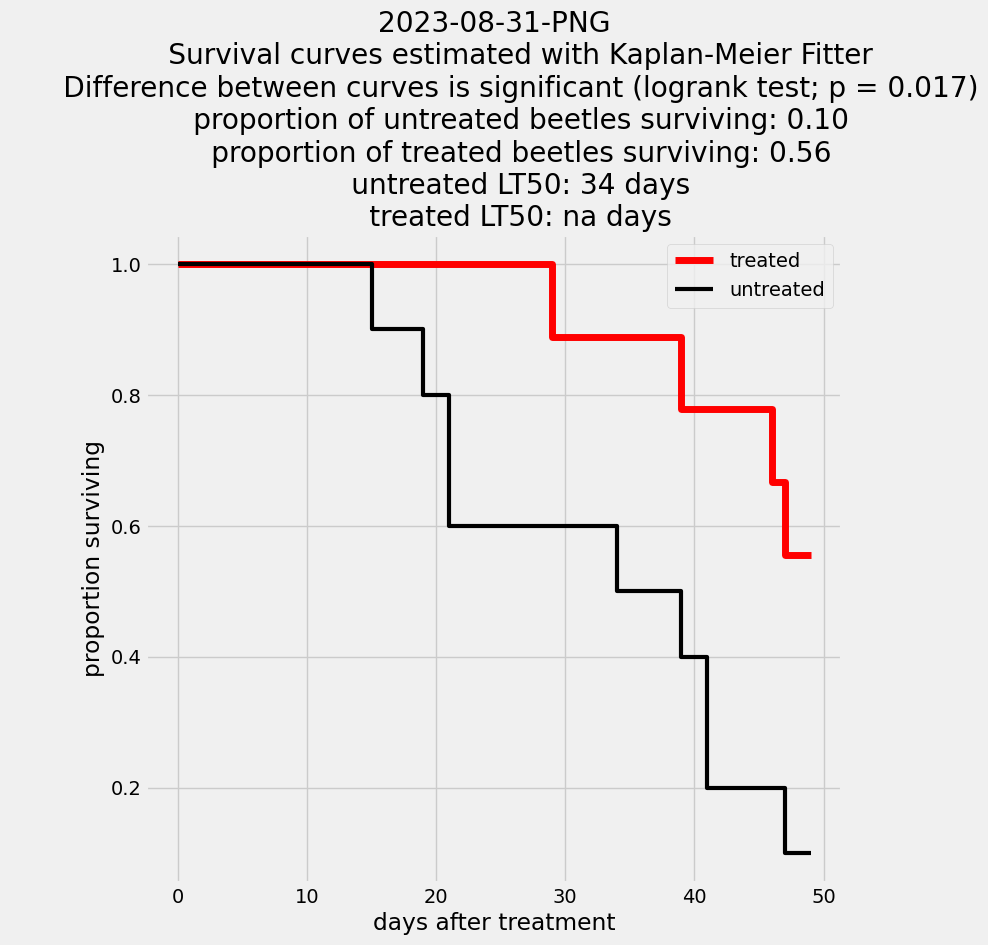
\includegraphics[width=\textwidth]{images/survival_curves/2023-08-31-PNG}
		\caption{Replcate 3.}
	\end{subfigure}
	\caption{Survival curves for bioassays of OrNV isolate PNG.}
	\label{fig:PNG survival curves}
\end{figure}

% V23B survival curves

\begin{figure}[h]
	\centering
	\begin{subfigure}{.3\textwidth}
		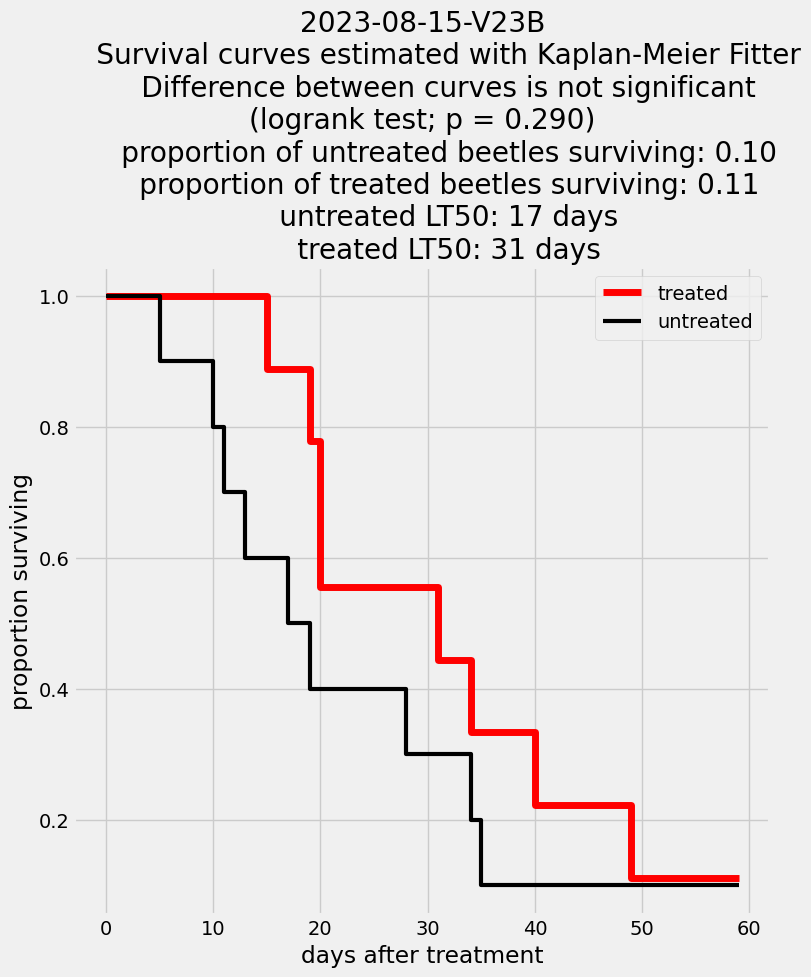
\includegraphics[width=\linewidth]{images/survival_curves/2023-08-15-V23B}
		\caption{Replicate 1.}
	\end{subfigure}
	\begin{subfigure}{.3\textwidth}
		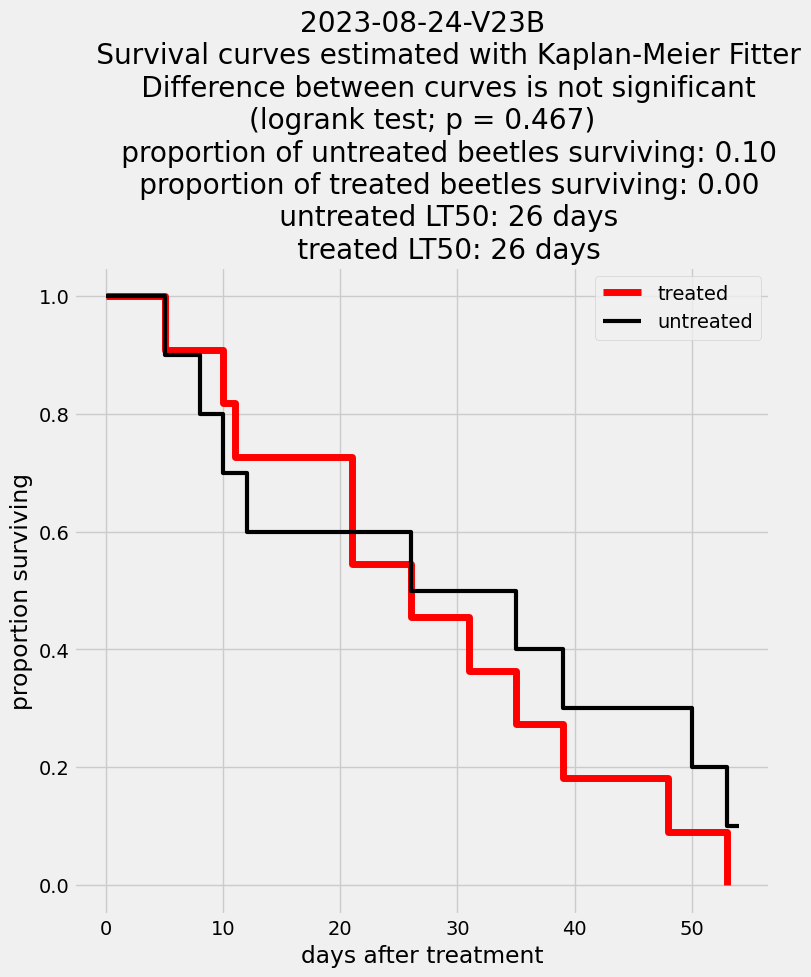
\includegraphics[width=\textwidth]{images/survival_curves/2023-08-24-V23B}
		\caption{Replicate 2.}
	\end{subfigure}
	\begin{subfigure}{.3\textwidth}
		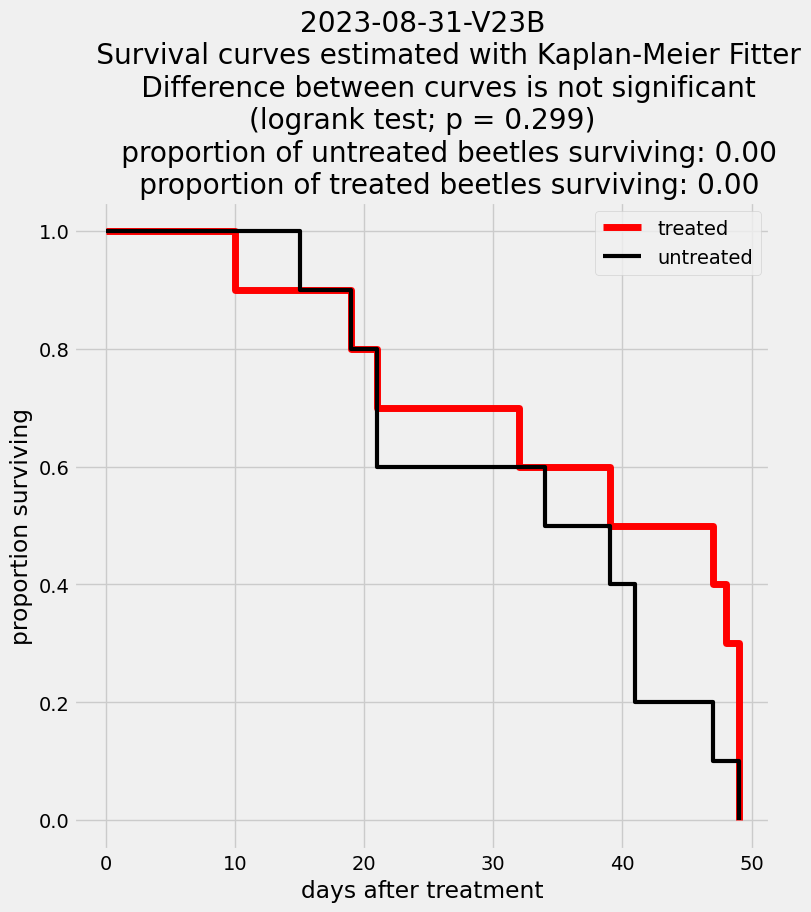
\includegraphics[width=\textwidth]{images/survival_curves/2023-08-31-V23B}
		\caption{Replcate 3.}
	\end{subfigure}
	\caption{Survival curves for bioassays of OrNV isolate V23B.}
	\label{fig:V23B survival curves}
\end{figure}

% X2B survival curves

\begin{figure}[h]
	\centering
	\begin{subfigure}{.3\textwidth}
		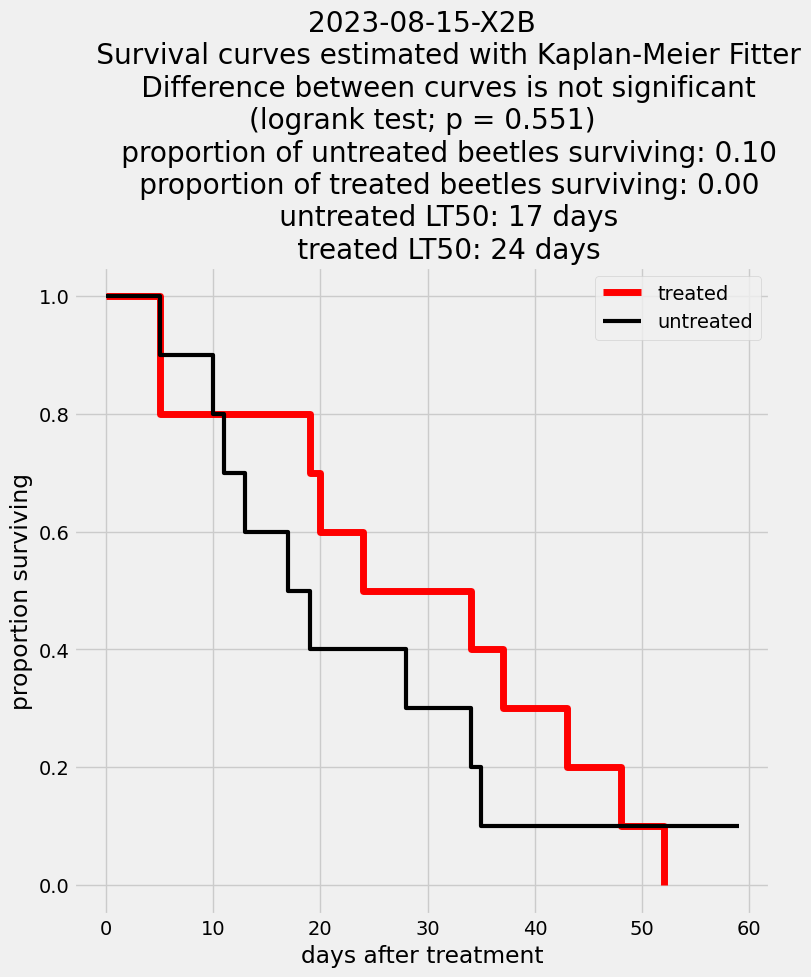
\includegraphics[width=\linewidth]{images/survival_curves/2023-08-15-X2B}
		\caption{Replicate 1.}
	\end{subfigure}
	\begin{subfigure}{.3\textwidth}
		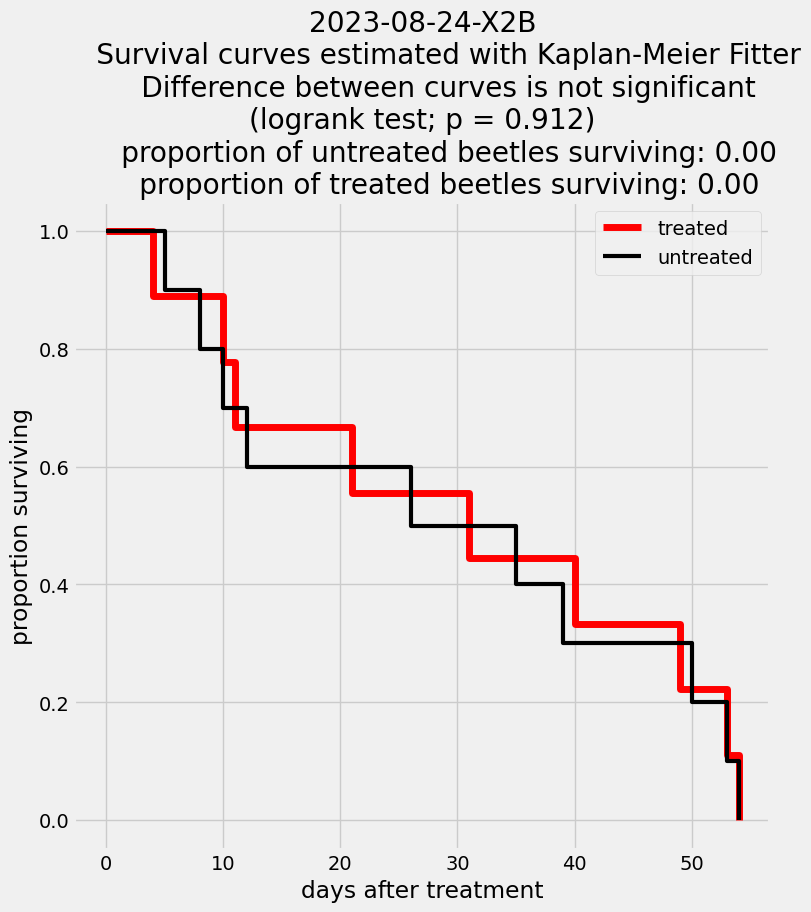
\includegraphics[width=\textwidth]{images/survival_curves/2023-08-24-X2B}
		\caption{Replicate 2.}
	\end{subfigure}
	\begin{subfigure}{.3\textwidth}
		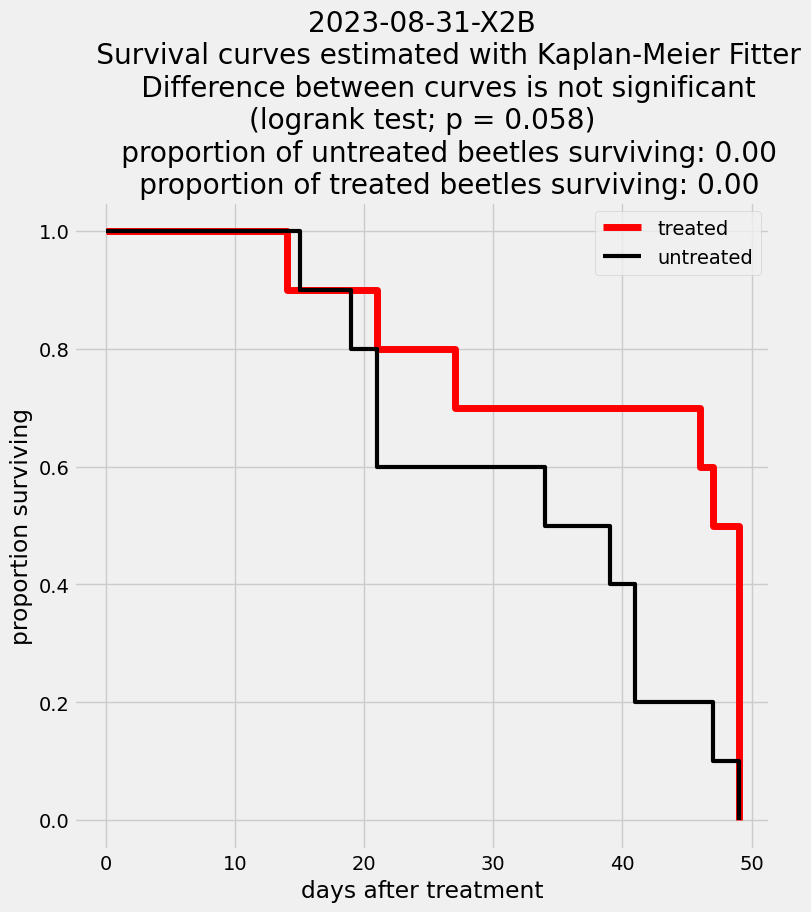
\includegraphics[width=\textwidth]{images/survival_curves/2023-08-31-X2B}
		\caption{Replcate 3.}
	\end{subfigure}
	\caption{Survival curves for bioassays of OrNV isolate X2B.}
	\label{fig:X2B survival curves}
\end{figure}

\clearpage
\paragraph{Post mortem observations}

\paragraph{Heartbeat.} Many beetles which were deemed dead because they had stopped moving their legs were actually alive. 45\% of beetles examined during post mortems had heartbeats. These heartbeats were evident as movement beneath the dorsum only after elytra had been removed.  

\paragraph{Mites.} 23\% of beetles harbored mites commonly seen during CRB rearing.

\paragraph{Nematodes.} On August 14, 2023 while doing postmortem examinations of adult beetles which died in these assays, we detected nematodes on the dorsal surface of the abdomen of a dead beetle. \href{https://www.youtube.com/shorts/dKVup7q7FF0}{Click here} to see a YouTube video of the original discovery. This is the first record for nematodes associated with CRB on Guam \cite{Moore2023nematodes}.

Since then, we have observed that 60\%  of dead or dying adult beetles from the bioassays have been infested with nematodes (Fig. \ref{fig:nematode2}). Most of the time, these are observed underneath the elytra or on the ventral surface of the abdomen. Numbers range from a few to hundreds of nematodes per beetle. On several occasions, nematodes were observed swimming within the hemocoel.

These nematodes have not been identified and we do not know if they are entomopathogens which may be useful biological control agents.

% TODO: \usepackage{graphicx} required
\begin{figure}[H]
	\centering
	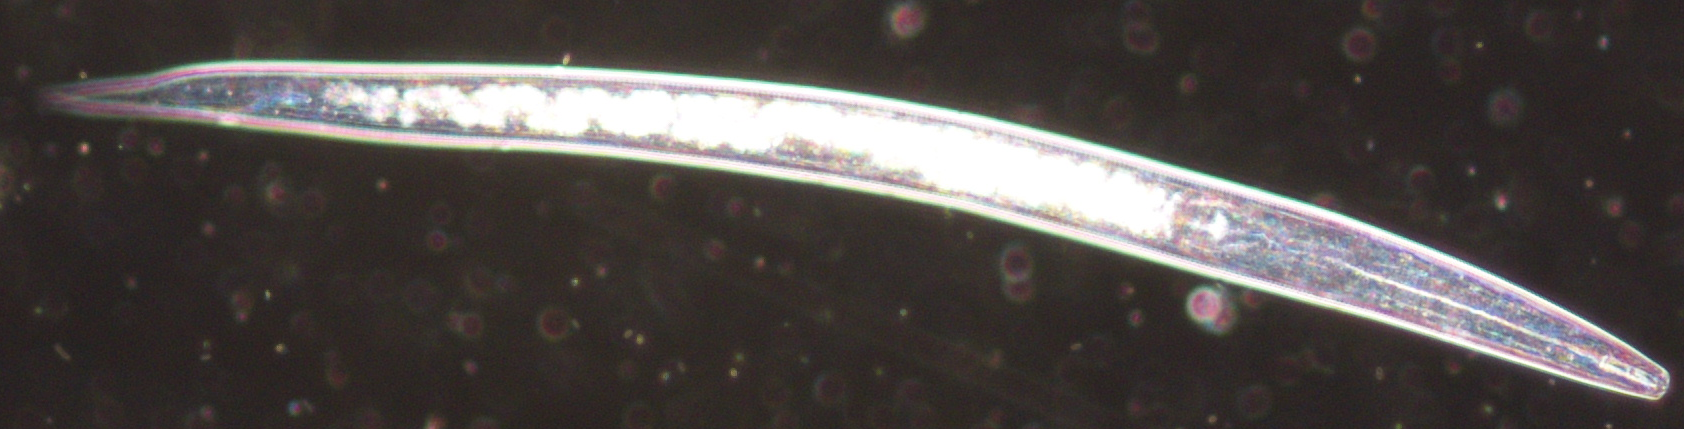
\includegraphics[width=0.7\linewidth]{images/nematode2}
	\caption{Nematode collected from beneath elytra of an adult coconut rhinoceros beetle, \textit{Oryctes rhinoceros}. Length is 0.36 mm.}
	\label{fig:nematode2}
\end{figure}

\begin{table}[H]
	\centering
	\caption{Percent of post mortem observations in which mites, nematodes and heartbeat were present.}
	\label{ornv detection}

	\begin{tabular}{lrrr}
		\hline
		treatment &  mites &  nematodes &  heartbeat \\
		\hline
		CONTROL &         25 &        50 &             50 \\
		DUG42 &         33 &        66 &             46 \\
		PNG &         22 &        63 &             40 \\
		V23B &         26 &        61 &             50 \\
		X2B &          9 &        54 &             40 \\
		\hline
		Mean & 23 & 60 & 45 \\
		\hline
	\end{tabular}
\end{table}


\clearpage

\paragraph{Dosage}.

% TODO: \usepackage{graphicx} required
\begin{figure}[h]
	\centering
	\caption{Distribution of OrNV doses consumed by CRB adults used in bioassays. The target dose of 40,000 IU is indicated be the red line. 77 beetles consumed less than the target dose and 61 consumed more than the target dose.}
	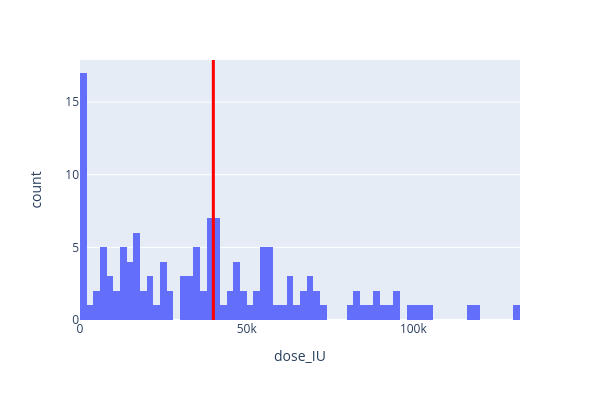
\includegraphics[width=0.7\linewidth]{images/dosage_distribution}
	\label{fig:dosagedistribution}
\end{figure}



\paragraph{OrNV detection}

Only a small proportion of gut samples sent to AgResearch New Zealand have been processed because a physical move to a new facility caused delays. Preliminary results (Table \ref{ornv detection}) indicate that all specimens belong to the CRB-G clade and beetles dosed with all 4 OrNV isolates resulted in infection.

\begin{table}[H]
	\centering
	\caption{OrNV detection.}
	\label{ornv detection}
	\begin{tabular}{lcc}
		\hline
		treatment  & \multicolumn{2}{c}{OrNV detection} \\ \cline{2-3}
		& Negative & Positive \\
		\hline
		CONTROL    & 34 & 1 (3\%) \\
		DUG42      & 19 & 10 (34\%) \\
		PNG        & 12 & 4 (25\%) \\		
		V23B       & 9  & 10 (53\%) \\
		X2B        & 13 & 4 (24\%) \\
		\hline
	\end{tabular}
\end{table}

\begin{figure}[H]
	\centering
	\begin{subfigure}{.49\textwidth}
		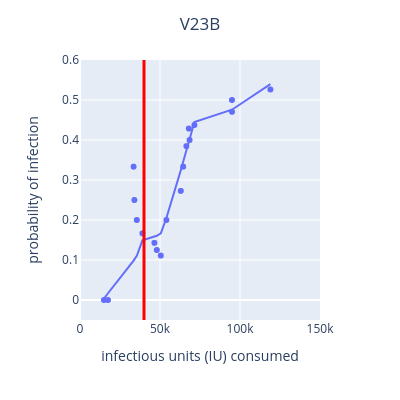
\includegraphics[width=\linewidth]{images/V23B_infection_probability.png}
	\end{subfigure}
	%\hfill
	\begin{subfigure}{.49\textwidth}
		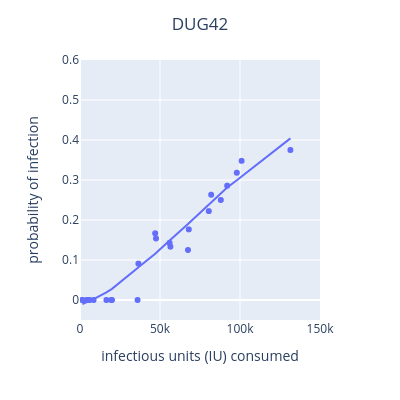
\includegraphics[width=\textwidth]{images/DUG42_infection_probability.png}
	\end{subfigure}
	%\hfill
	\begin{subfigure}{.49\textwidth}
		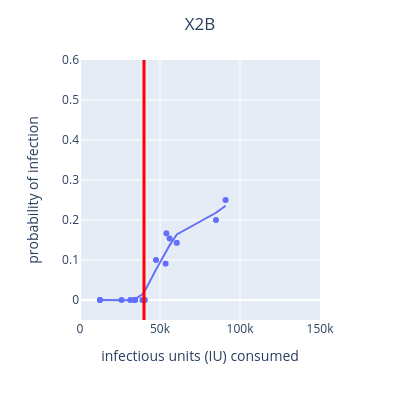
\includegraphics[width=\textwidth]{images/X2B_infection_probability.png}
	\end{subfigure}
	%\hfill
	\begin{subfigure}{.49\textwidth}
		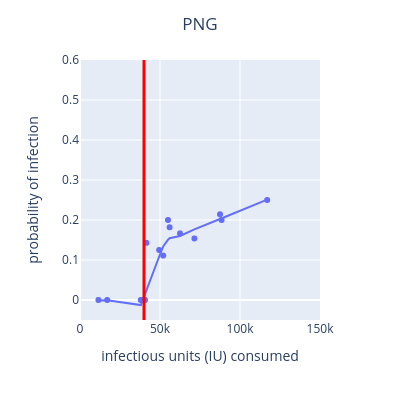
\includegraphics[width=\textwidth]{images/PNG_infection_probability.png}
	\end{subfigure}
	\caption{Relationship between dose and probability of infection in Guam CRB-G adults.}
	\label{fig:infection probability}
\end{figure}

\clearpage
\section{Objective 3:  Establish Island-wide Monitoring Systems for CRB and Coconut Palm Health}
\label{monitoring}

\begin{framed}
The CRB-G outbreak on Guam is currently unmonitored on an island-wide basis. An island-wide pheromone trapping system, using about 1500 traps, was operated by the University of Guam from 2008 to 2014. This monitoring system was transferred to the Guam Department of Agriculture which abandoned the effort at the end of February, 2016.  Currently, many coconut palms are being killed by CRB-G. But, in the absence of a monitoring system, we do not have an estimate of tree mortality or whether or not the damage is increasing or decreasing. Clearly, establishment of a monitoring system is necessary to evaluate success of the proposed biocontrol project, or any other mitigation efforts. We intend to re-establish island-wide trapping and to establish a sustainable roadside video survey which uses artificial intelligence to detect CRB damage in dash-cam videos. 
\end{framed}

\subsection{Objective 3a: Pheromone Traps}

%\begin{framed}
%We plan to installed 150 CRB pheromone monitoring traps. These will be baited with oryctalure and serviced semimonthly. These traps catch approximately equal numbers of males and females which remain alive in the traps for several weeks. Collected beetles will be used for autodissemination of virus and a subsample will be used for virus detection. Traps will be deployed at least 3 months prior to initiation of autodissemination.  
%
%A web database already exists for Guam CRB trap data and it is available for use by this project (URL: \url{https://mysql.guaminsects.net}; database: \textbf{oryctes}; user: \textbf{readonlyguest}; password: \textbf{readonlypassword}; main tables: \textbf{trap} (2,265 records) and \textbf{trap\_visit} (89,114 records)).
%\end{framed}

\subsubsection{Previously reported progress}

We have not deployed new pheromone traps. But we continue to maintain trap lines in central Guam, at the Leo Palace Resort, and in northern Guam, at the University of Guam Agricultural Station in Yigo.

\subsubsection{Recent progress}

We maintain 35 pheromone traps at the Leo Palace Resort Golf Course. These are serviced biweekly. The main purpose of this activity is to provide adult beetles for experiments.

We have decided not to use pheromone traps for island-wide monitoring because we don't know the relationship between trap catch and CRB population density. Mark-release-recapture studies show that the commercially available pheromone, oryctalure, is not highly attractive to CRB-G on Guam \cite{siderhurstEffectsUltravioletLight2021}. The recapture rate for 567 marked beetles released in the vicinity of pheromone traps was only 11\%.

We will continue to use automated roadside image surveys as a cost-effective instead of pheromone traps for island-wide monitoring of CRB on Guam. 



\clearpage
\subsection{Objective 3b: Roadside Damage Surveys}

\begin{framed}
Damage symptoms such as v-shaped cuts to fronds, bore holes, and dead standing coconut palm stems are readily observed during roadside surveys. Survey data will be collected on a smart-phone dash-cam app which georeferences each image. Initially, images of coconut palm damage by CRB-G will be detected, classified and tagged by a technician. When a large number of images have been tagged, these will be used to train an object detector. This work will result in a fully automated CRB damage detection and monitoring system which generates detection alerts and damage maps. This automated system will be useful as an early detection device for CRB. Roadside surveys on Guam will be performed bimonthly and the system will also be tested on Tinian, an island just north of Guam on which CRB has never been detected.

The envisioned system has already been successfully prototyped. A custom object detector for CRB damage has been trained using the TensorFlow implementation of the Faster R-CNN Deep Learning model (Moore, unpublished).
\end{framed}

\subsubsection{Previously reported progress}

Bimonthly automated roadside video surveys for CRB damage are now operational on Guam and the system has been tested on Rota. Videos recorded with a smart phone attached to a vehicle are analyzed using custom-designed artificial intelligence software which recognizes coconut palms and measures CRB damage. A nontechnical description of the survey method is given in the next section.

A presentation on this new CRB survey methodology was made at the December 9 2020 meeting of the CRB-G Action Group conducted as a Zoom webinar. Videos of all presentations at this meeting are available online \cite{mooreVideoRecordingCRBG2020}.

\clearpage
\paragraph{Guam Roadside Video Survey 1}

The following four images were extracted from a draft of the University of Guam's Western Pacific Tropical Research Center impact report for 2020. They provide a nontechnical overview of the new automated roadside video survey for CRB damage and results from the first Guam survey in October, 2020.

\begin{figure}[h]
	\centering
	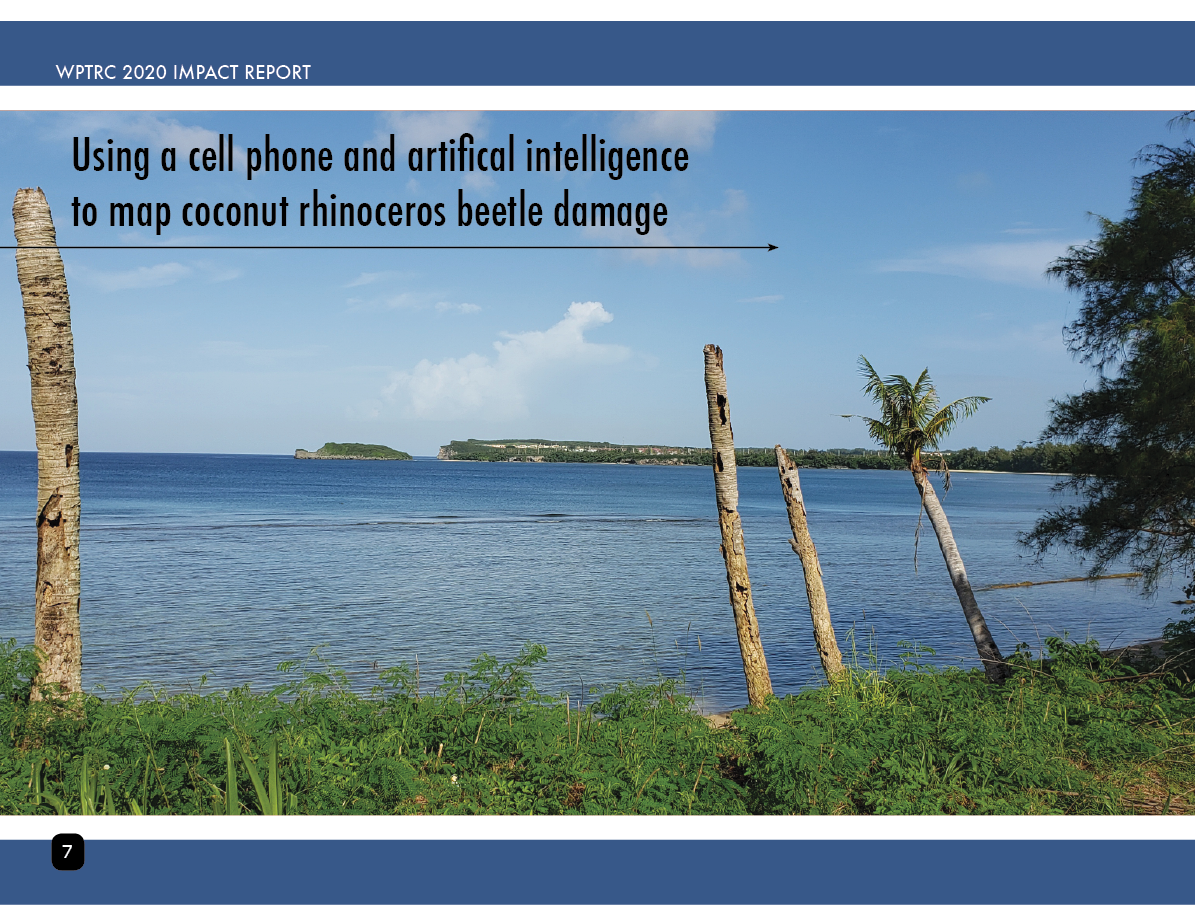
\includegraphics[width=1\linewidth]{images/impact-report07.png}
	\caption{Feature article in the University of Guam's Western Pacific Tropical Research Center impact report for 2020.}
	\label{fig:roadside1-1}
\end{figure}

\begin{figure}[h]
	\centering
	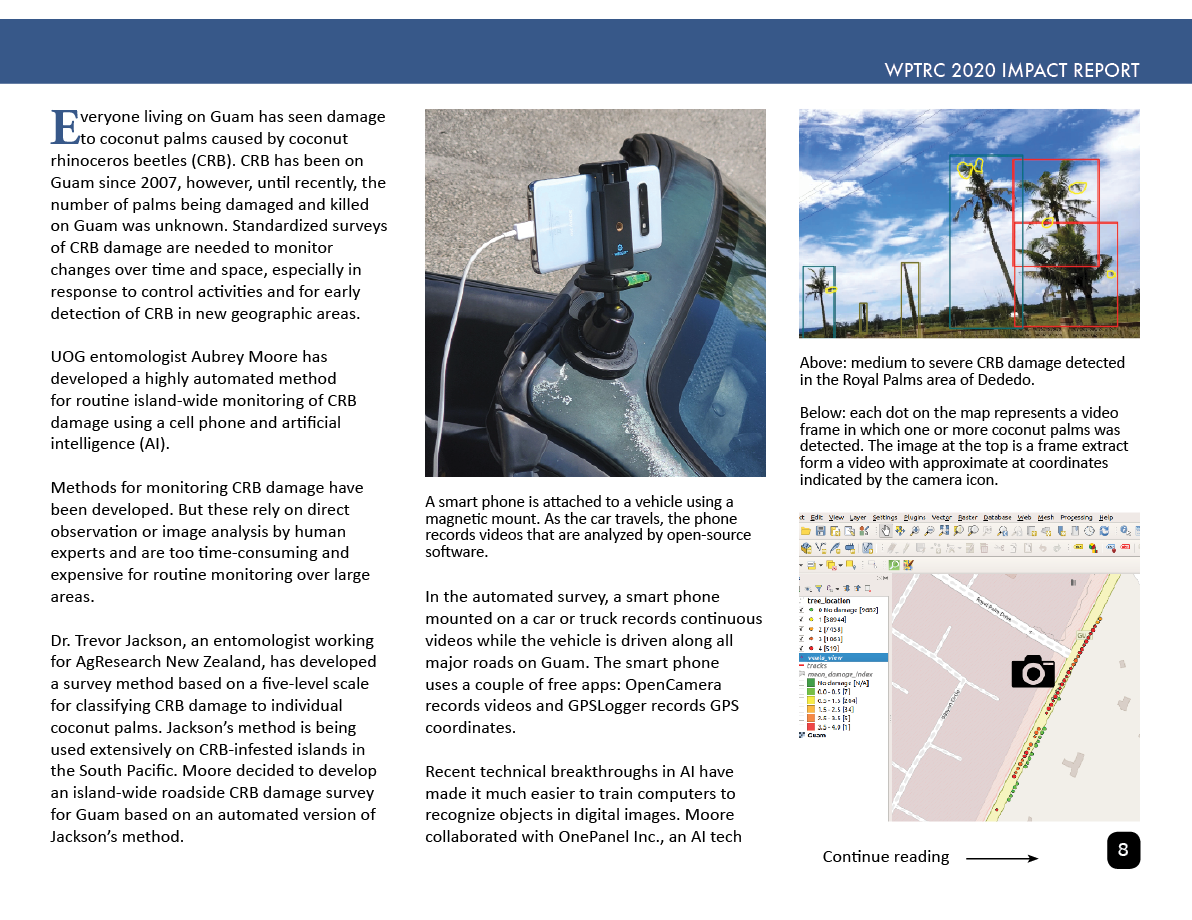
\includegraphics[width=1\linewidth]{images/impact-report08.png}
	\caption{[Continued] Feature article in the University of Guam's Western Pacific Tropical Research Center impact report for 2020.}
	\label{fig:roadside1-2}
\end{figure}

\begin{figure}[h]
	\centering
	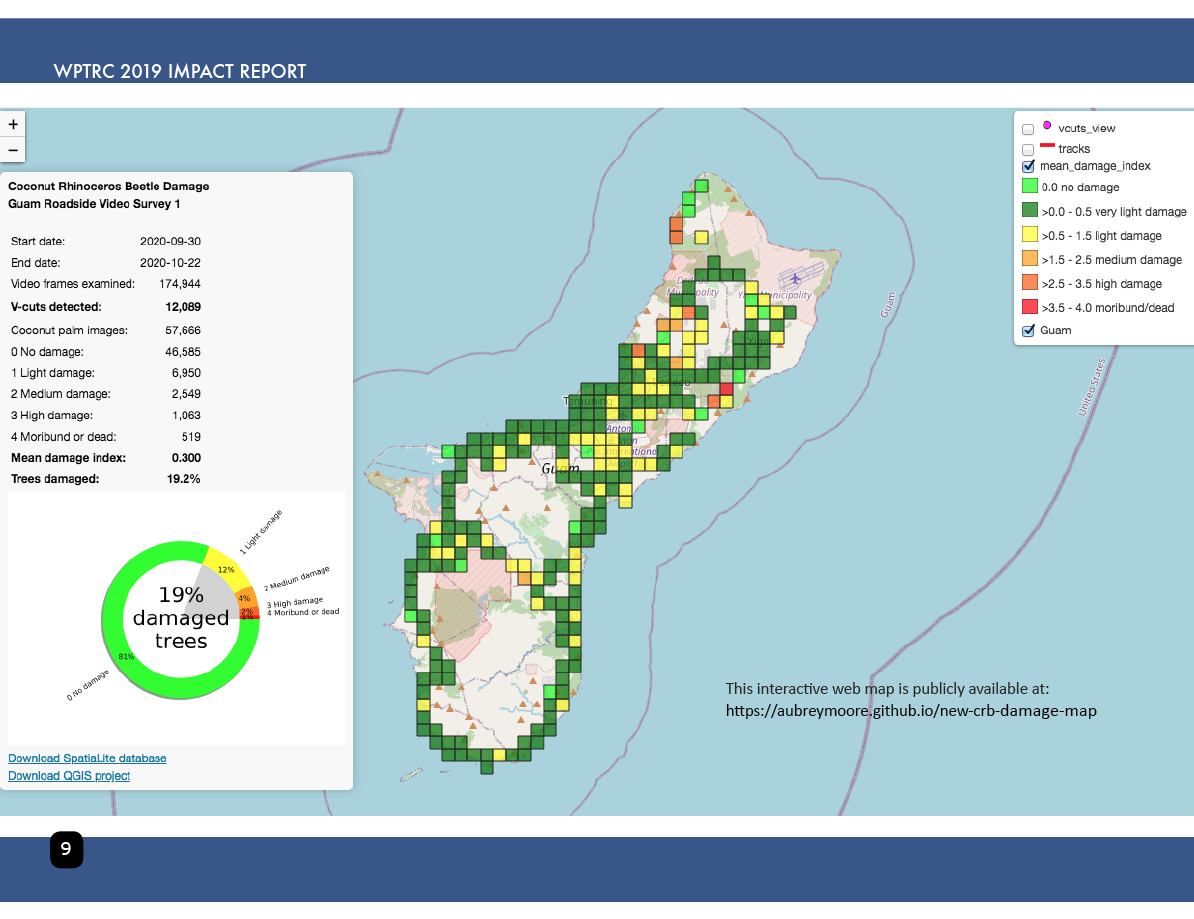
\includegraphics[width=1\linewidth]{images/impact-report09.png}
	\caption{[Continued] Feature article in the University of Guam's Western Pacific Tropical Research Center impact report for 2020. This interactive web map is publicly avaiable at: \url{https://aubreymoore.github.io/new-crb-damage-map}}
	\label{fig:roadside1-3}
\end{figure}

\begin{figure}[h]
	\centering
	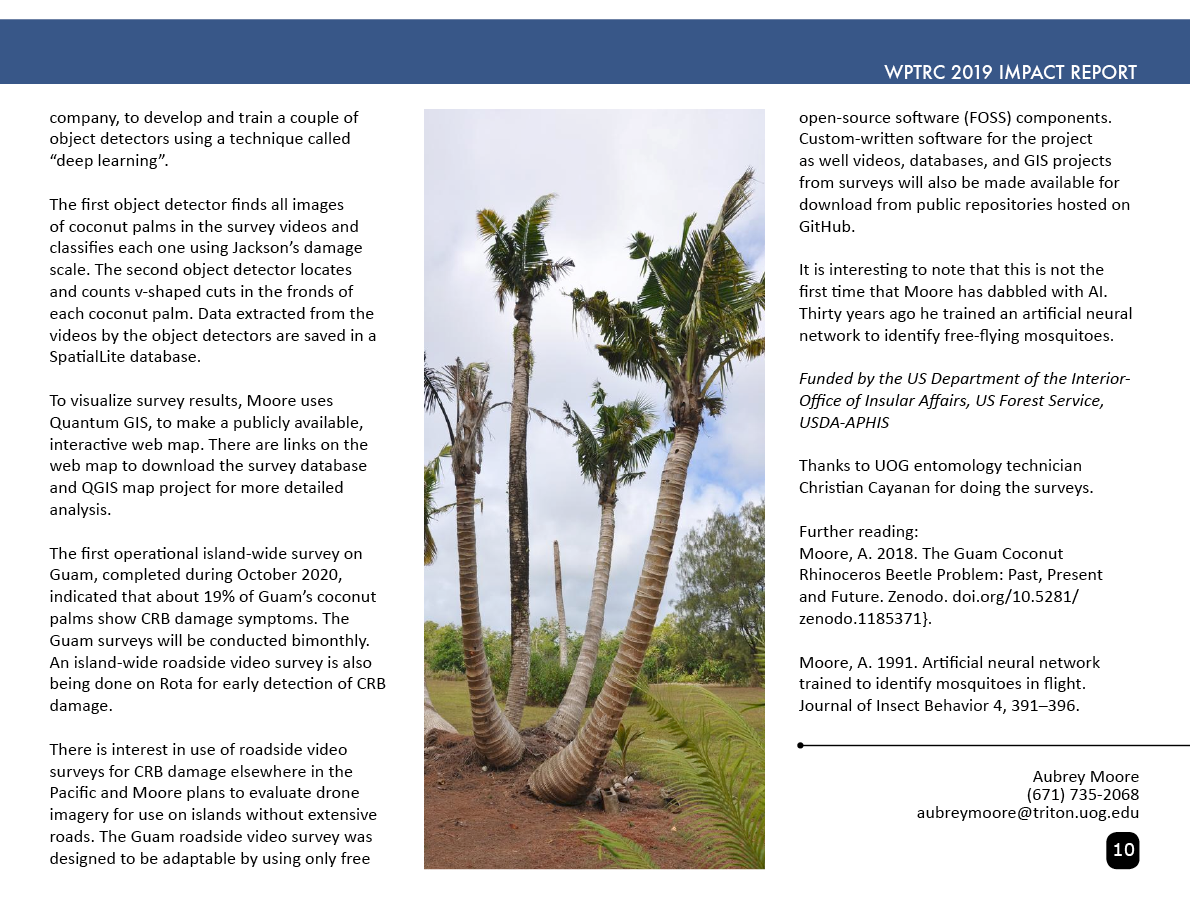
\includegraphics[width=1\linewidth]{images/impact-report10.png}
	\caption{[Continued] Feature article in the University of Guam's Western Pacific Tropical Research Center impact report for 2020.}
	\label{fig:roadside1-4}
\end{figure}

%\clearpage
%\paragraph{Guam Roadside Video Survey 2}
%
%The proportion of coconut palms damaged by CRB increased significantly from 19.2\% in
%October 2020 to 21.5\% in December 2020 (p < 0.001; Fisher's exact test).
%
%\begin{figure}[h]
%	\centering
%	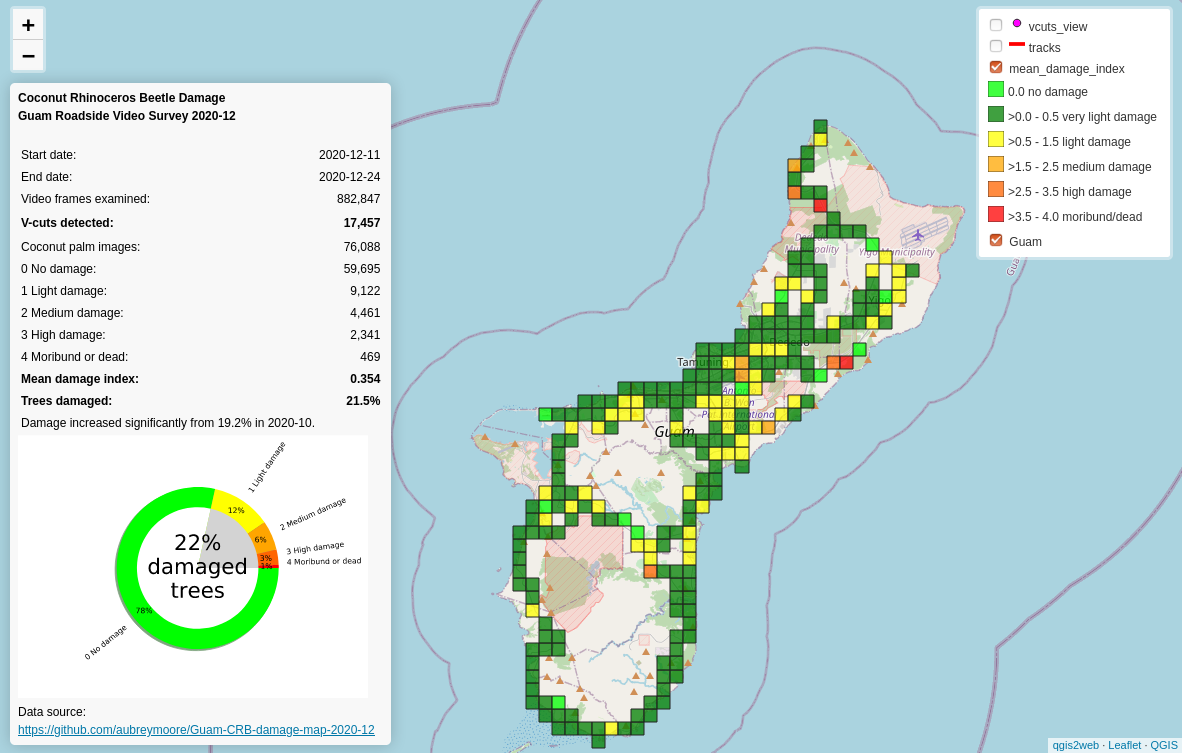
\includegraphics[width=1\linewidth]{../images/crb-webmap-2020-12.png}
%	\caption{Screenshot of an interactive web map of results from a roadside video survey of
%		CRB damage on Guam in December 2020 \url{https://aubreymoore.github.io/Guam-CRB-damage-map-2020-12/webmap/v1/}.}
%	\label{fig:guam02}
%\end{figure}


\clearpage
\paragraph{Rota Roadside Video Survey 1}

Rota was invaded by CRB in 2017 and eradication efforts by Rota Department of Land and Natural Resources have successfully kept the population at a very low level, although the population has begun to spread to new areas of the island. In October 2020, a smart phone and associated equipment was sent to Rota-DLNR so that they could do an initial roadside video survey in support of their CRB control efforts. In addition to the equipment, a survey setup guide \cite{mooreSetAutomatedRoadside2020} and a setup video \cite{mooreYouTubeVideoMounting2020} were prepared and sent.
 
The survey was performed by Mark Mangolana, Rota-DLNR and the phone containing videos from the survey was returned to the University of Guam.  Videos were analyzed using the workflow developed for the Guam surveys. The resulting web map contained many false positives for CRB damage, but there is one hit which shows a classic v-shaped cut probably caused by CRB. For convenience, data for this hit (images, date, location) were documented as an iNaturalist observation (Figure \ref{fig:rota-inat-obs}). If this v-shaped cut was caused by CRB, there will be a bore hole. Rota-DLNR are following up to see if this is the case.


\begin{figure}[h]
	\centering
	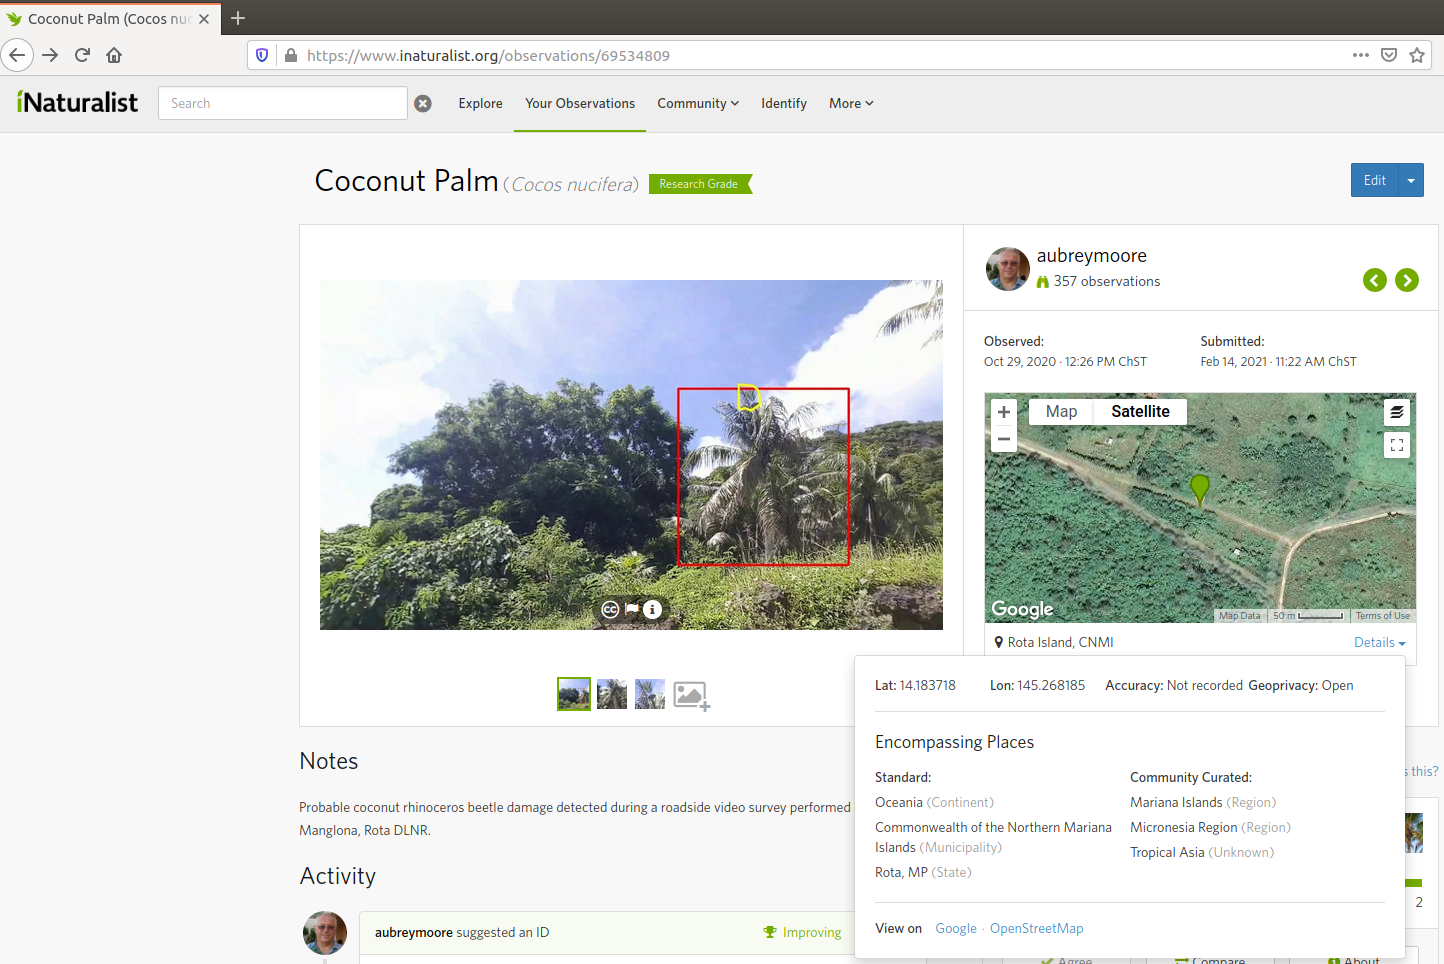
\includegraphics[width=1\linewidth]{images/Rota-iNat-obs}
	\caption{Screenshot of an iNaturalist observation documenting probable coconut rhinoceros beetle damage detected during a roadside video survey performed by Rota DLNR. \url{https://www.inaturalist.org/observations/69534809}.}
	\label{fig:rota-inat-obs}
\end{figure}

\clearpage

\subsubsection{Roadside CRB Damage Assessments on Guam}

We continue to monitor CRB damage on Guam using automated roadside image surveys. We also continue to improve our survey methods. Processing was simplified by changing our raw data format from videos taken at 15 images per second to georeferenced still images taken at 1 image per second. This reduced data file memory requirements by 93\% and we no longer need to rely on a second smart phone app to record latitude and longitude.

To date, 10 island-wide CRB damage surveys of Guam have been completed. An \href{https://github.com/aubreymoore/Guam-CRB-web-maps}{index of web maps and related data} is maintained a GitHub web page. This page shows changes in damage levels over time (Fig. \ref{fig:timeline}) and links to web maps such as one for the latest damage survey completed on 2023-09-22 (Fig. \ref{fig:webmap-2023-09-22}).

\begin{figure}[H]
	\centering
	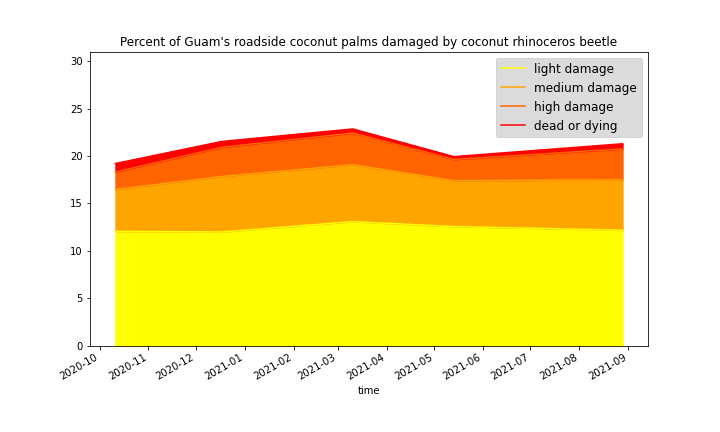
\includegraphics[width=\linewidth]{images/timeline}
	\caption{Changes in CRB damage over time.}
	\label{fig:timeline}
\end{figure}

\begin{figure}[H]
	\centering
	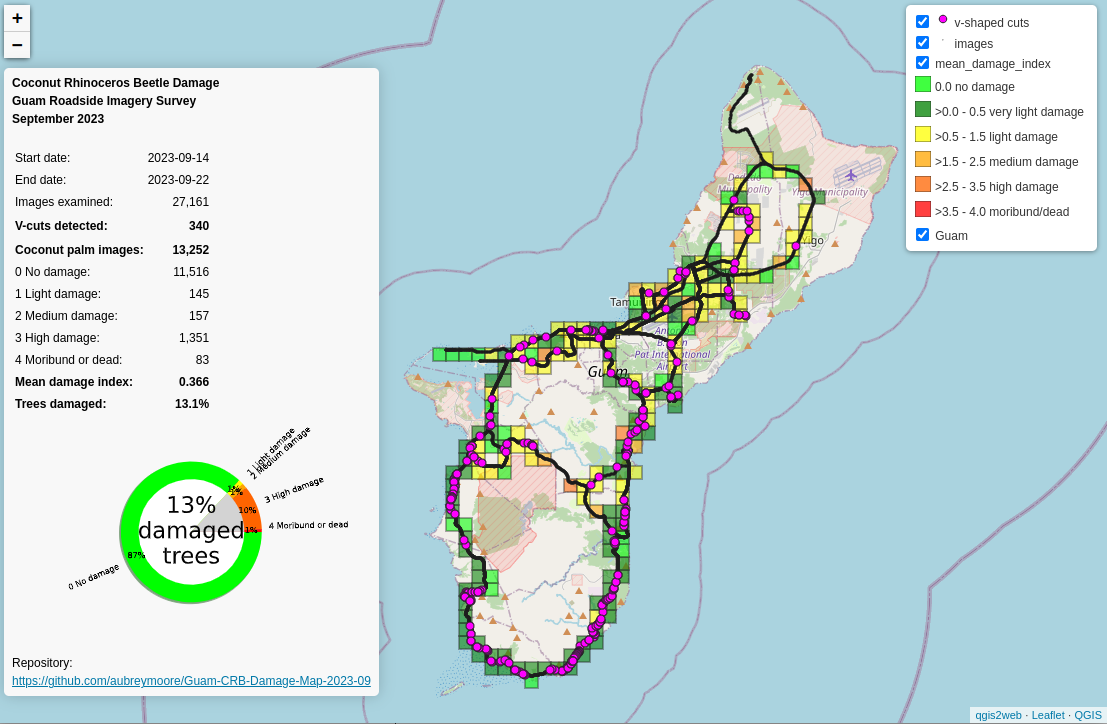
\includegraphics[width=\linewidth]{images/crb-webmap-2023-09-22}
	\caption{Screen capture of an online interactive map of coconut rhinoceros beetle damage on Guam. \url{https://aubreymoore.github.io/Guam-CRB-Damage-Map-2023-09/webmap/}.}
	\label{fig:webmap-2023-09-22}
\end{figure}

In addition to using our methods for routine monitoring of CRB damage, they can be used for early detection of CRB. An initial test of this idea was done on Rota and results were reported in a webinar organized by the Department of the Interior - Office of Insular Affairs  \cite{usdepartmentoftheinterior-officeofinsularaffairsYouTubeVideoCoconut2021}.

Software tools developed for our automated roadside damage monitoring can be used to detect CRB damage in digital images from any source. Recently, an object detector which we trained to find characteristic v-shaped cuts caused by CRB to examine web images was used to find evidence for an unconfirmed report of CRB establishment in Mexico \cite{jacksonSocialMediaPosts2022}. We were successful (Fig.  \ref{fig:crb-mexico}).

\clearpage
\subsubsection{Roadside CRB damage assessment on Majuro, Republic of the Marshall Islands. Oct. 7, 2023}

A few days after coconut rhinoceros beetle was detected on Majuro, Christian Cayanan from the University of Guam visited the island to perform an automated roadside survey of CRB damage using methods developed on Guam. The survey was performed from 11 am and 3 pm on October 7, 2023. A smart phone programmed to record a georeferenced HD images at a rate of once per second was attached to the outside of a vehicle. The vehicle which was driven the eastern tip of the island to the western tip, returning along the same route. 13,488 roadside images were recorded.

These images were examined by a pair of object detectors, one which detected coconut palms and one which detected v-shaped cuts to fronds which are distinctive symptoms of CRB adult feeding damage. Results were reported in the form of an \href{https://aubreymoore.github.io/Majuro-CRB-Damage-Map-2023-10/webmap/#12/7.1098/171.2099}{interactive web map}. 

The original webmap reported a much higher level of damage on Majuro than expected. Examination of images showed that the object detectors were generating many false-positive detections. The data were reanalyzed. The detection threshold was increased from 50\% to 70\% for the coconut palm detector and from 50\% to 99\% for the v-shaped cut detector. In addition all detected v-shaped cuts were examined visually.

A \href{https://aubreymoore.github.io/Majuro-CRB-damage-map-1/webmap/#12/7.1082/171.2072}{revised interactive web map} has was generated. This map shows only 3 v-shaped cuts tightly clustered at a location just east of the airport.

At this point, the object detectors are not very efficient and results require validation by human observers viewing images or making field observations. The coconut palm detector makes few mistakes. But the v-shaped cut detector generates many false-positives and false-negatives. Further training and tuning of both detectors is needed. However, even in the current state, the methodology is still quite useful. Data acquisition is not a problem: acquiring 13,488 images required only 4 hours and the computer workflow reduced the human labor dramatically. It was not necessary to view 13,488 images, but only to validate a few hundred images selected by the object detectors. Details of the Majuro survey are available in \href{https://aubreymoore.github.io/Majuro-tech-report-20231201/Majuro-tech-report.pdf}{this technical report}.  

%![](web-screenshot.png)
%
%**Figure 1** Screen capture of an online interactive map of coconut rhinoceros beetle damage on Guam. <https://aubreymoore.github.io/Guam-CRB-Damage-Map-2021-08/webmap>
%
%![](timeline.pdf)
%
%**Figure 2** Changes in CRB damage over time.

\begin{figure}[H]
	\centering
	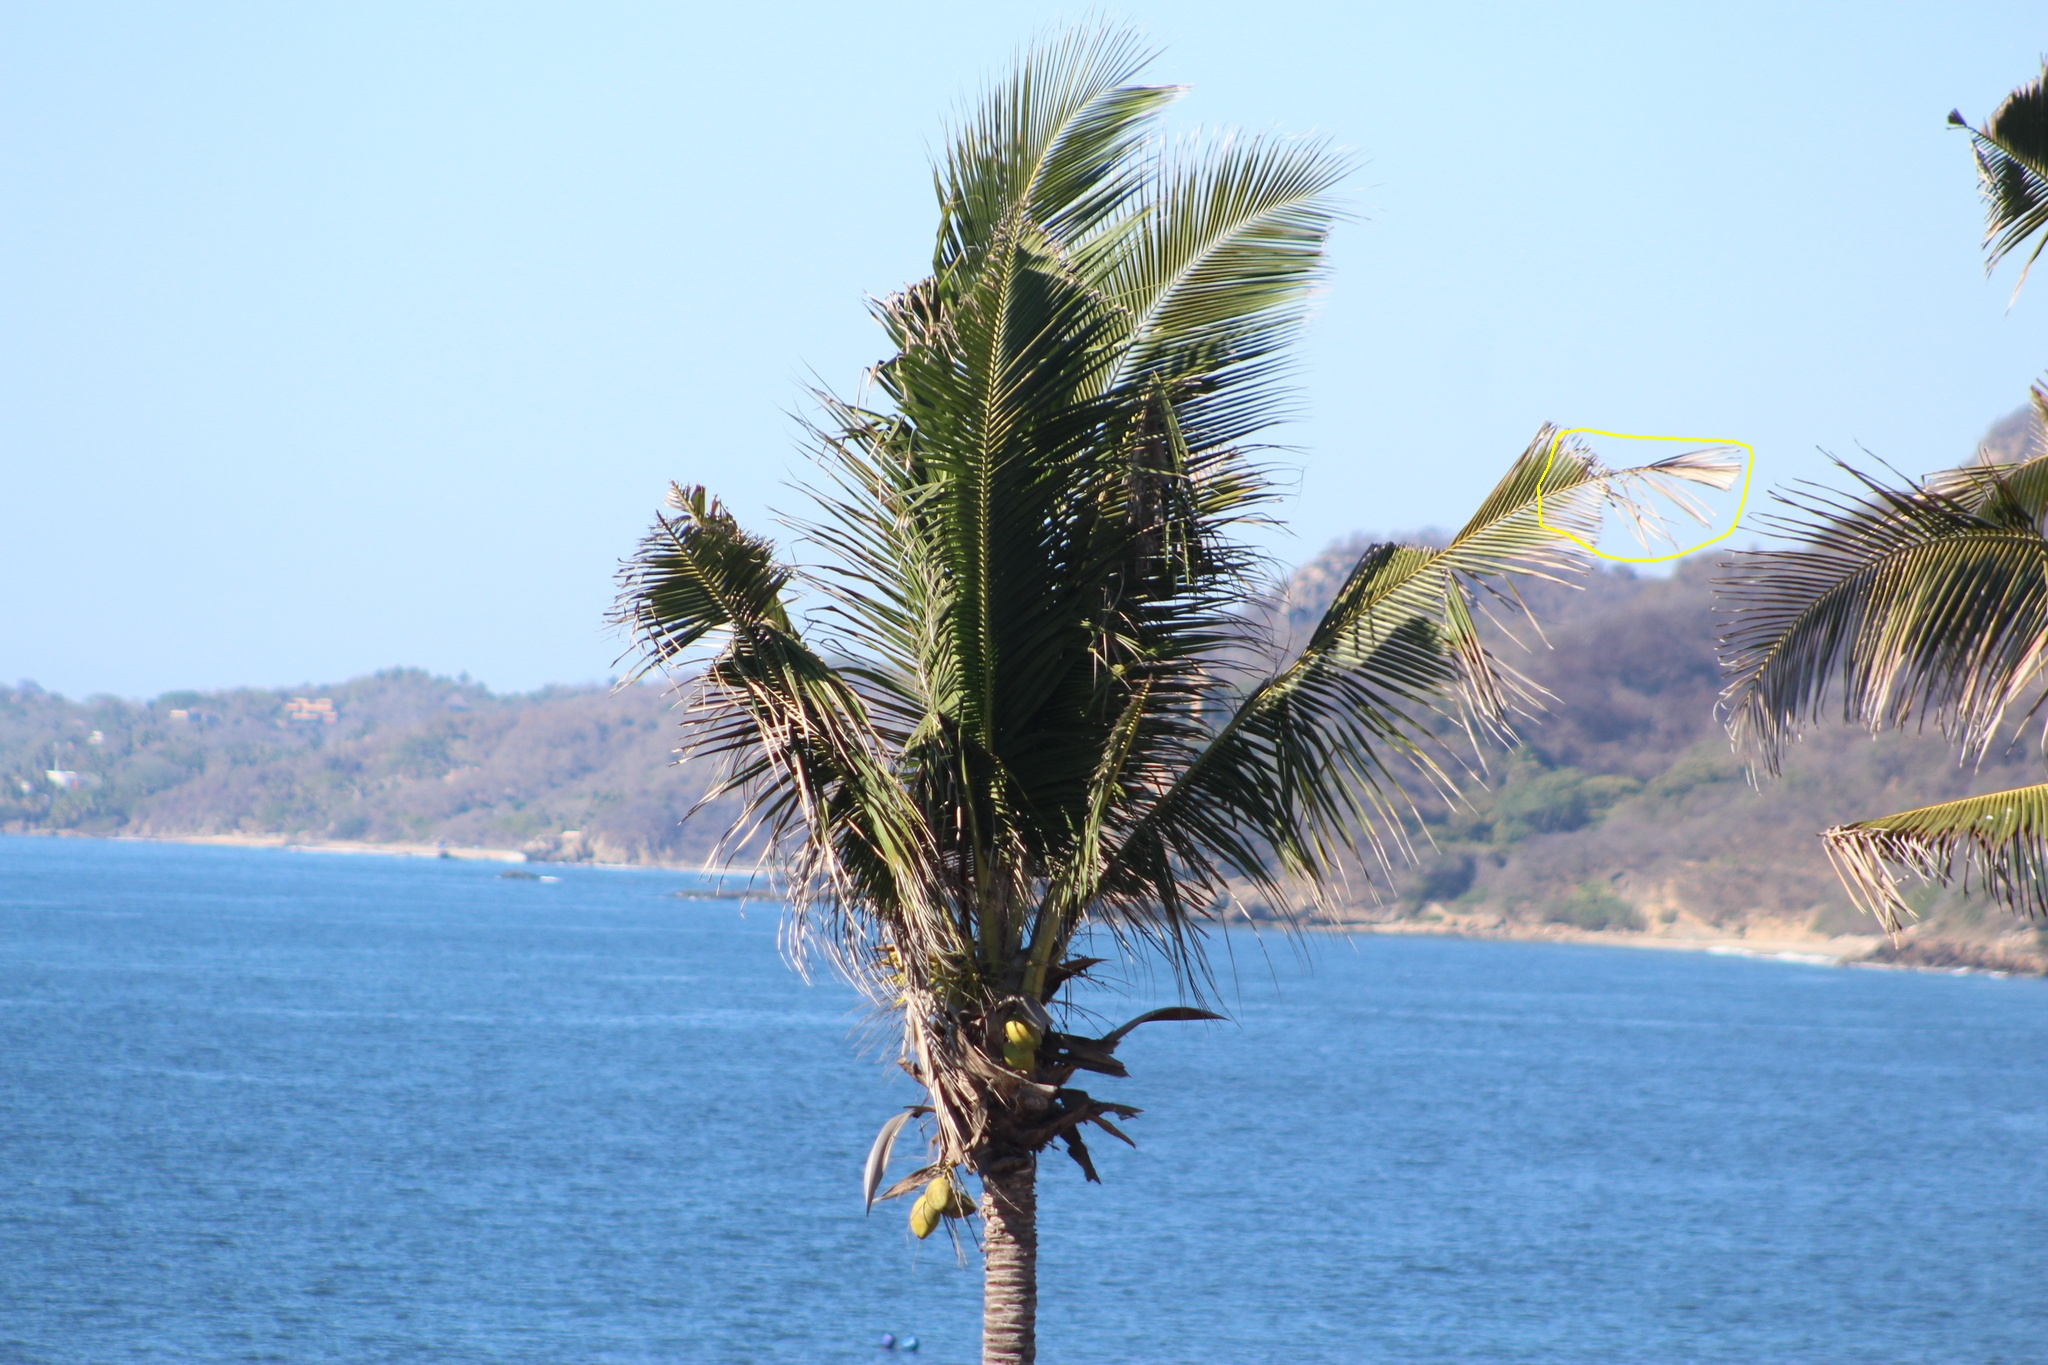
\includegraphics[width=\linewidth]{images/crb-mexico}
	\caption{Coconut palm in Mexico with CRB damage symptoms. This image was selected by an automated search of web images using an object detector developed for CRB damage monitoring on Guam. Image source: \url{https://www.inaturalist.org/observations/76810823}.}
	\label{fig:crb-mexico}
\end{figure}

\clearpage

\section{Related Activities and Recent Progress}

\subsection{Forest Insect and Disease Leaflet (FIDL) for Coconut Rhinoceros Beetle}

The PI is first author on a Forest Service FIDL for CRB. Available online at: \\
\begin{footnotesize}
\url{https://www.fs.usda.gov/foresthealth/docs/fidls/FIDL-191-CoconutRhinocerosBeetle.pdf} 
\end{footnotesize}

\subsection{Using Harmonic Radar to Detect CRB Breeding Sites}

Effective control of CRB requires location and destruction of larval breeding sites which my occur anywhere were there is an accumulation of decaying plant material. Previously, we successfully tracked radio-tagged CRB adults to find cryptic breeding sites. But high cost of radio transmitters and limited battery capacity made this method too expensive for regular use. We suggest that harmonic radar tags may be a cost-effective replacement for miniaturized radio transmitters and have published a journal article on this idea \cite{mooreProposalDetectingCoconut2022}. Harmonic radar tags do not require a battery, are very inexpensive (about \$2 per tag) and have unlimited shelf and field life.

A field trial was funded by Forest Service grant 20-DG-11052021-227.
During July 2023, Dr. Siderhurst and two of his students, Skylar List and Theodore Yoder, traveled to Guam to perform this trial. We constructed harmonic radar tags by attaching antennae to diodes using conductive silver paint and glue. These tags were then glued onto pronota of CRB adults. Sixty-four out of 101 tagged CRB flew out of containers set up at 2 field sites. Unfortunately, we were not able to detect any of these beetles during ground-based searches using harmonic radar detectors. For details, see \href{https://github.com/aubreymoore/Harmonic-Radar/blob/master/final-report-202212/final-report-202212.pdf}{the project's final report}. 

Examination of 36 beetles which failed to fly showed that most (22 of them) had antennae wires which had detached from diodes. We think that conductive silver paint and glue may not be strong enough for attachment of nitinol antenna wires to tags applied to CRB because these large beetles are very energetic and their movements cause breakage of the connections between diodes and nitinol wire antennae. 

\subsubsection{Improved Harmonic Tag Construction Method}

We are currently attempting to solve this problem by attaching antenna wires to diodes using a special solder and flux combination design specifically for nitinol wire. We are very lucky that Michael Jordan of the US Forest Service who is stationed on Guam has very specialized skills in soldering miniature electronic components which he developed while serving in the US Navy.

Specialized soldering equipment and flux designed specifically for nitinol were purchased. New tags were constructed (Fig. \ref{fig:harmonicradartags}), but these have not yet been tested in a new field trial.

% TODO: \usepackage{graphicx} required
\begin{figure}[H]
	\centering
	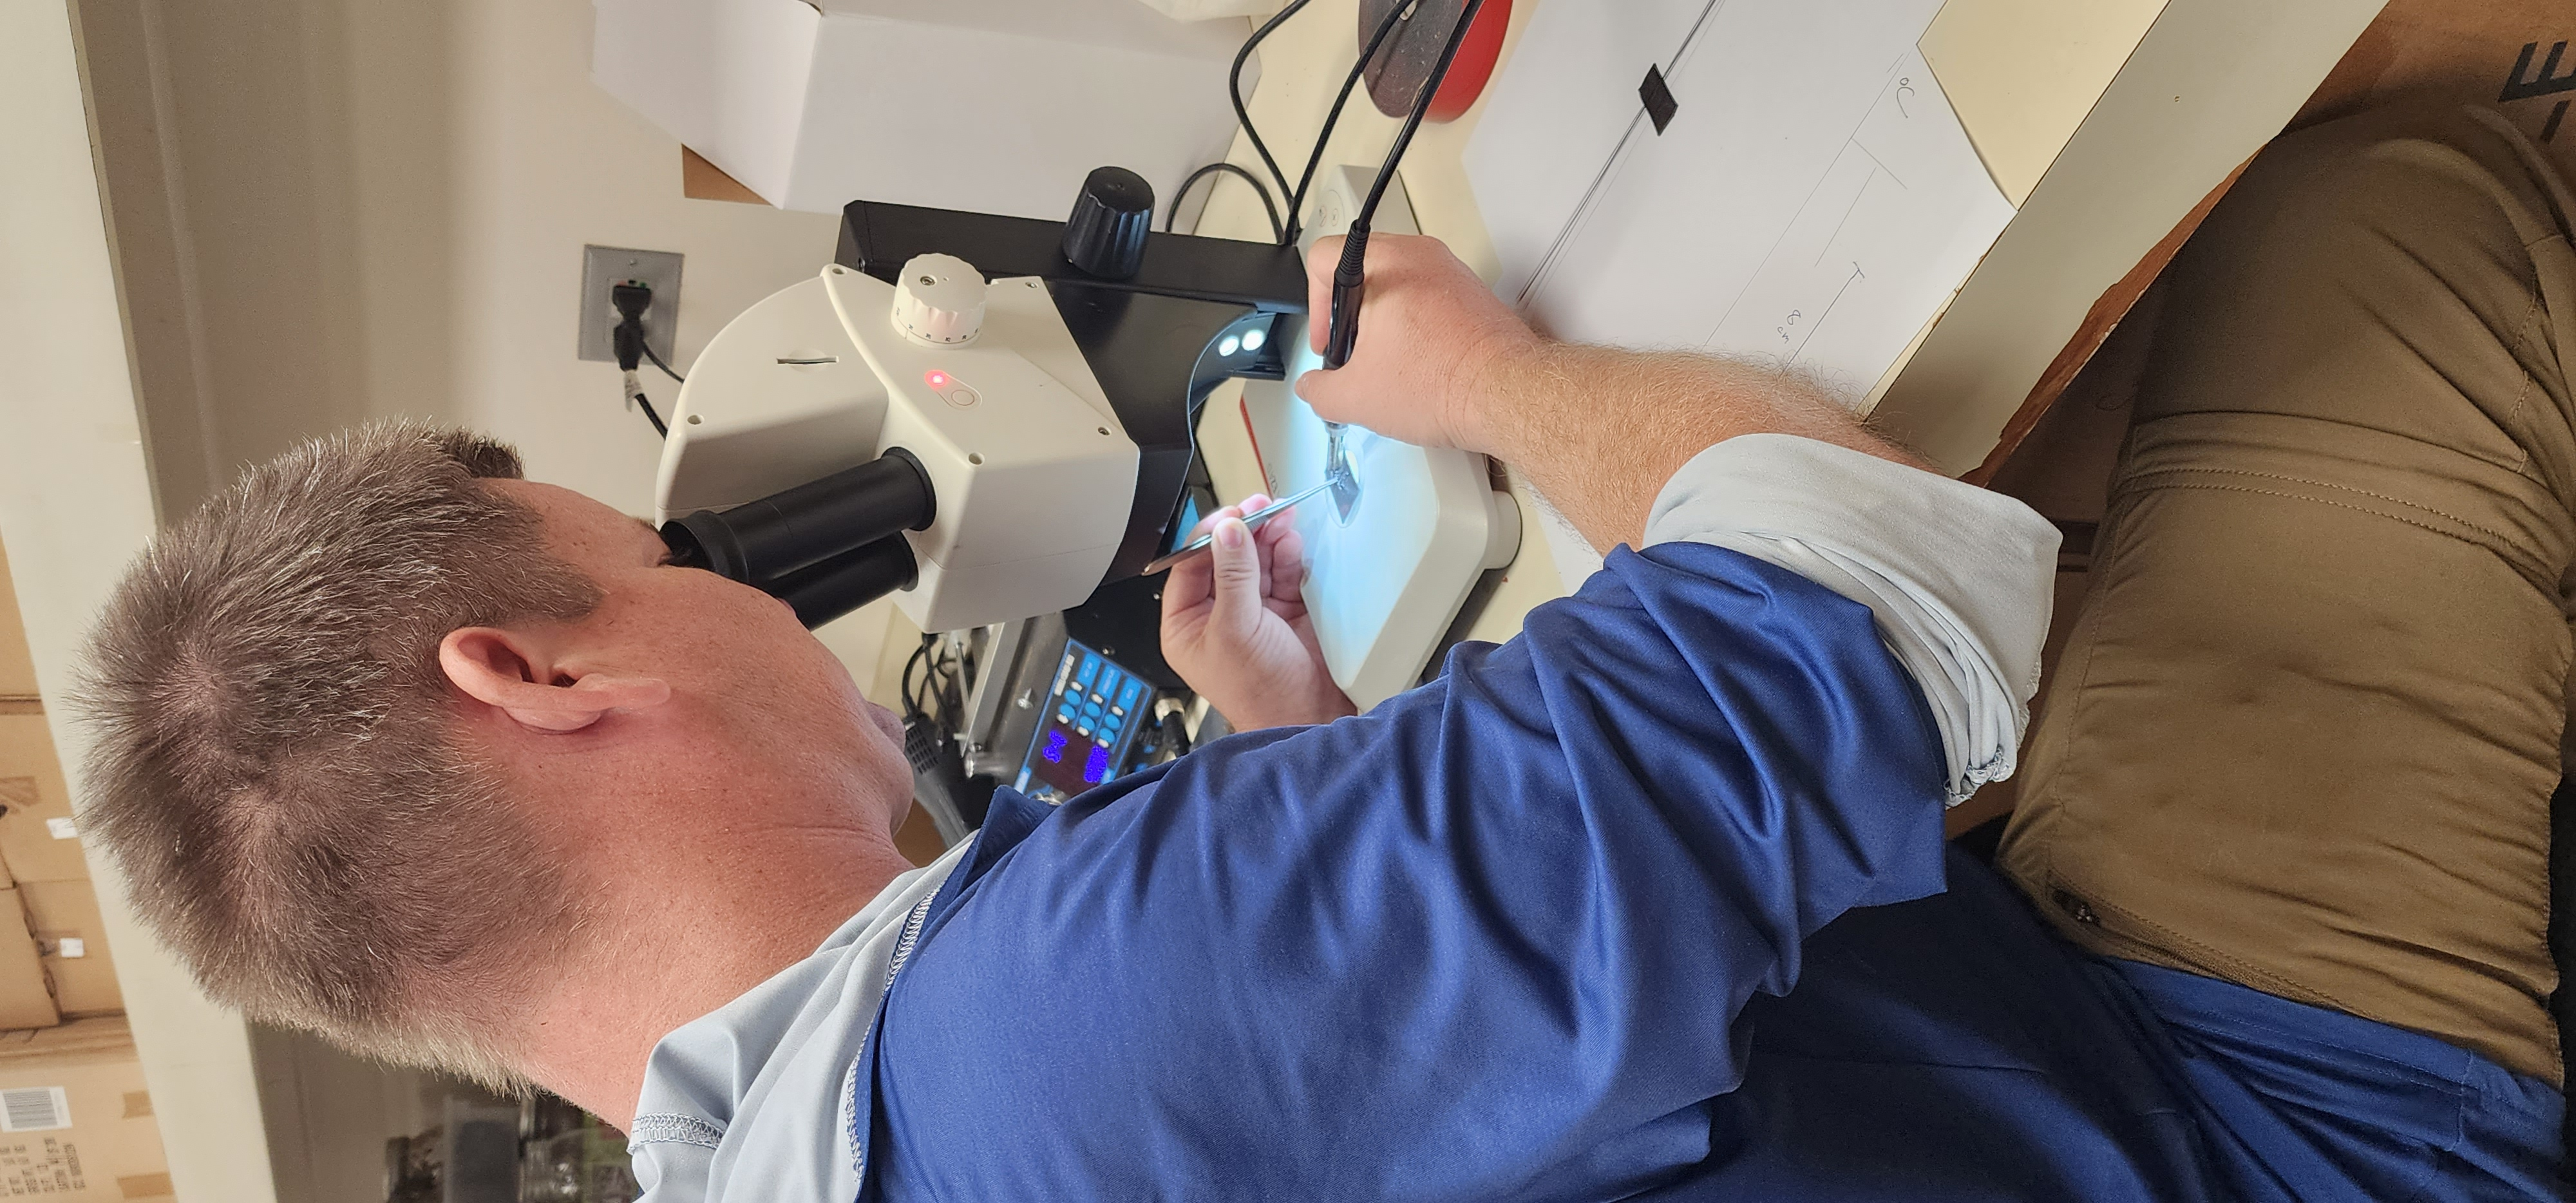
\includegraphics[angle=-90,origin=c,width=0.6\linewidth]{images/harmonic_radar_tags}
	\caption{Michael Jordan, US Forest Service, soldering nitinol antennae wires onto harmonic radar diodes.}
	\label{fig:harmonicradartags}
\end{figure}

\clearpage
\subsection{Role of Symbionts in Rearing CRB}

In attempt to speed up development of CRB grubs in our rearing program, we added frass from third instar larvae into larval medium (sterilized finely ground material from dead standing coconut stems). Weight gain was significantly improved (Fig. \ref{fig:symbiontmass}). However, survival mortality remained low (Fig. \ref{fig:symbiontsurvival}).



% TODO: \usepackage{graphicx} required
\begin{figure}[H]
	\centering
	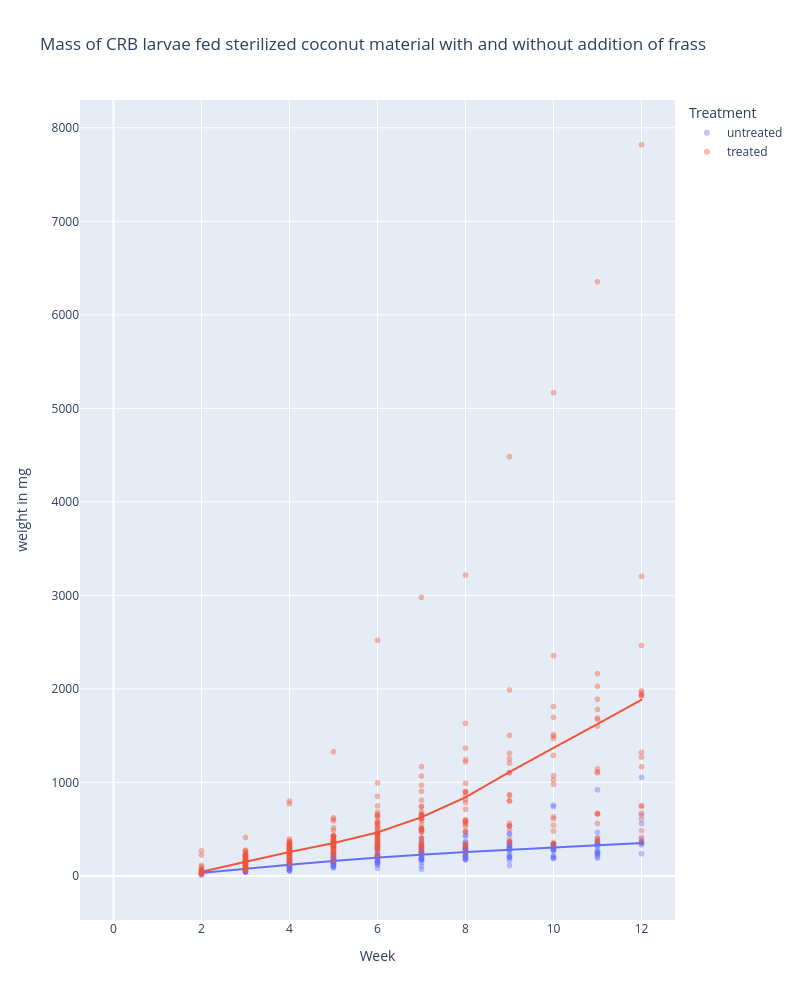
\includegraphics[width=0.8\linewidth]{images/symbiont_mass}
	\caption{}
	\label{fig:symbiontmass}
\end{figure}

% TODO: \usepackage{graphicx} required
\begin{figure}[H]
	\centering
	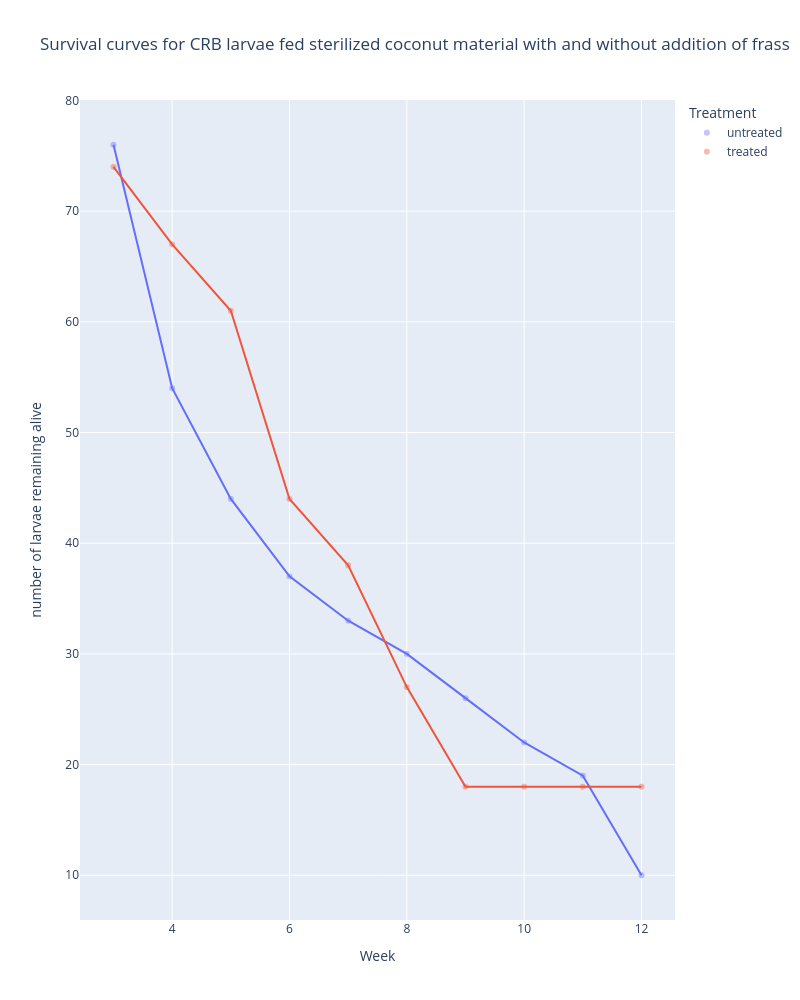
\includegraphics[width=0.8\linewidth]{images/symbiont_survival}
	\caption{}
	\label{fig:symbiontsurvival}
\end{figure}

\newpage

\printbibliography

\end{document}
